\chapter{线性映射}

在前几讲的学习中,我们从开始的 8 条运算性质出发,利用这些线性运算的特点导出线性扩张与子空间的关联,然后经过线性相关性的讨论最终得到线性空间的本质结构实际上就是可以由基经过一系列线性运算扩张而来,因此我们对线性空间的研究很多时候只需要研究其基和维数即可,由此我们对线性空间的研究和描述就可以转为研究基和维数——这是线性空间的基本结构属性. 当然我们最后也讨论了线性空间之间的运算. 从本讲开始我们将研究不同线性空间之间的关联,我们的手段是定义两个线性空间之间的线性映射,引出线性映射基本定理以及至今为止最重要的概念——同构,从而发掘出比较不同线性空间之间最本质的差别是什么,使我们的抽象更深一层,从而为之后我们在抽象的制高点将抽象转化为具象,讨论矩阵这一对线性映射的``有形''描述和线性映射本身的联系做准备.

\section{线性映射的定义}

\subsection{线性映射的定义}

\begin{definition}{线性映射}{线性映射的定义} \index{xianxingyingshe@线性映射 (linear map)}
    从线性空间$V_1(\mathbf{F})$到$V_2(\mathbf{F})$的一个映射$\sigma$是线性的,如果$\forall \alpha,\beta \in V_1$和$\forall \lambda,\mu \in \mathbf{F}$都有
    \begin{equation}\label{eq:5:线性映射}
        \sigma(\lambda\alpha+\mu\beta)=\lambda\sigma(\alpha)+\mu\sigma(\beta).
    \end{equation}

    从线性空间$V$到自身的线性映射$\sigma$也叫作$V$上的\term{线性变换},在有的教材中也称为\term{算子}\index{xianxingyingshe!xianxingbianhuan@线性变换 (linear transformation), 算子 (operator)}. 从线性空间$V(\mathbf{F})$到域$\mathbf{F}$的线性映射$f$叫作$V$上的线性泛函(或称线性函数,线性形式)\index{xianxingyingshe!xianxingfanhan@线性泛函 (linear functional)}.

    为方便称呼,我们称对于$V_1(\mathbf{F})$到$V_2(\mathbf{F})$的线性映射$\sigma$,$V_1(\mathbf{F})$是其出发空间,$V_2(\mathbf{F})$是其到达空间,也可简记为$\sigma: V_1\to V_2$.
\end{definition}
实际上,上述定义式 \ref*{eq:5:线性映射} 可以分拆为以下二式:
\begin{gather}
    \tag{加性} \sigma(\alpha+\beta)=\sigma(\alpha)+\sigma(\beta) \\
    \tag{齐次性} \sigma(\lambda\alpha)=\lambda\sigma(\alpha)
\end{gather}
这就是我们之前定义的同态性质,因此线性映射实际上就是线性空间之间的同态. 展开来说,线性映射将 $V_1$ 中的加法和数乘运算保留到 $V_2$ 中的加法和数乘运算,因为上述两式等号左边是 $V_1$ 中的运算,右边是 $V_2$ 中的运算.

根据定义,我们容易知道熟悉的过原点的一次函数是线性映射,而不过原点的一次函数不代表线性映射. 这似乎与平常的称呼不同,因为一次函数我们经常都称它们为``线性的'',这里我们必须强调的是,至少在线性代数的框架下,我们研究的``线性''性质是包含加性和齐次性两条要求的,事实上不过原点的一次函数我们可以视作非齐次线性方程,这里的``非齐次''的含义便很清晰了.

另一方面,如果我们不将一次函数视为映射,而将视为平面点集(不过原点的一条直线),我们可以回顾线性子空间中的描述,我们说过原点的直线构成平面的线性子空间,但不过原点的直线不是,我们判断的依据是不过原点的直线内的两点关于加法和数乘不封闭——仔细一想,是不是与线性映射定义中不满足加性、齐次性是同样的道理呢?

最后,我们需要强调一个非常容易被忽视但却很重要的一点. 事实上我们在\autoref{ex:运算与同构} 中关于$\mathbf{R}$与$\mathbf{R}^+$同构的讨论,以及坐标同构的讨论中已经引出了这一点,即线性映射$\sigma:V_1\to V_2$满足的表达式
\[\sigma(\alpha+\beta)=\sigma(\alpha)+\sigma(\beta)\]
中左边的加法是出发空间$V_1$中定义的加法运算,右边是到达空间$V_2$中定义的加法运算,二者并不是同一个加法,数乘也类似. %TODO: 同构

本小节最后我们讨论线性映射的两个重要的性质:
\begin{theorem}{}{线性映射零元性质}
    设$\sigma$是线性空间$V_1(\mathbf{F})$到$V_2(\mathbf{F})$的线性映射,则$\sigma(0_1)=0_2$.
\end{theorem}
注意定理中$0_1$为出发空间$V_1$中的零元,$0_2$代表到达空间$V_2$中的零元. 这只是为了区分两个空间零元而引入的记号,实际上下标也可以省略,直接写为0也可以.

\begin{proof}
    根据线性性,$\sigma(0+0)=\sigma(0)+\sigma(0)$,两边同时减去$\sigma(0)$可知$\sigma(0)=0$.
\end{proof}

\begin{theorem}{}{线性映射保相关性}
    设$\sigma$是线性空间$V_1(\mathbf{F})$到$V_2(\mathbf{F})$的线性映射,如果$V_1$中向量$\alpha_1,\alpha_2,\ldots,\alpha_n$线性相关,则$\sigma(\alpha_1),\sigma(\alpha_2),\ldots,\sigma(\alpha_n)$也线性相关.

    反之,若$\sigma(\alpha_1),\sigma(\alpha_2),\ldots,\sigma(\alpha_n)$线性无关,则$\alpha_1,\alpha_2,\ldots,\alpha_n$必线性无关.
\end{theorem}
这一性质表明线性映射保持线性相关性. 定理中两个描述互为逆否命题,因此我们可以只证明前者.

\begin{proof}
    设$\alpha_1,\alpha_2,\ldots,\alpha_n$线性相关,则存在不全为0的数$\lambda_1,\lambda_2,\ldots,\lambda_n$使得$\lambda_1\alpha_1+\lambda_2\alpha_2+\cdots+\lambda_n\alpha_n=0$,于是
    \[\sigma(\lambda_1\alpha_1+\lambda_2\alpha_2+\cdots+\lambda_n\alpha_n)=\lambda_1\sigma(\alpha_1)+\lambda_2\sigma(\alpha_2)+\cdots+\lambda_n\sigma(\alpha_n)=0\]
    因此存在不全为零的数$\lambda_1,\lambda_2,\ldots,\lambda_n$使得$\lambda_1\sigma(\alpha_1)+\lambda_2\sigma(\alpha_2)+\cdots+\lambda_n\sigma(\alpha_n)=0$,因此$\sigma(\alpha_1),\sigma(\alpha_2),\ldots,\sigma(\alpha_n)$线性相关.
\end{proof}

需要注意的是,线性映射可能将线性无关的向量组映射为线性相关的向量组,例如
\begin{example}{}{}
    设$\sigma$是线性空间$\mathbf{R}^2$到$\mathbf{R}^2$的线性映射,定义$\sigma(x,y)=(x+y,x+y)$,则$\sigma$将线性无关的向量组$(1,0),(0,1)$映射为线性相关的向量组$(1,1),(1,1)$.
\end{example}

\subsection{线性映射举例}

事实上,``线性性''在数学中是一个非常基本的性质,我们首先来看以下几个在数学中非常基本的概念,它们都是线性映射的例子:
\begin{example}{}{}
    数学分析与概率论中的线性映射:
    \begin{enumerate}
        \item (极限) $\displaystyle\lim_{n\to +\infty}(\lambda a_n+\mu b_n)=\lambda\lim_{n\to +\infty}a_n+\mu\displaystyle\lim_{n\to +\infty}b_n$;

        \item (求导) $(\lambda f(x)+\mu g(x))'=\lambda f'(x)+\mu g'(x)$;

        \item (积分) $\displaystyle\int_a^b(\lambda f(x)+\mu g(x))\,\mathrm{d}x=\lambda\int_a^bf(x)\,\mathrm{d}x+\mu\displaystyle\int_a^bg(x)\,\mathrm{d}x$;

        \item (数学期望) $\mathrm{E}(\lambda X+\mu Y)=\lambda \mathrm{E}(X)+\mu \mathrm{E}(Y)$.
    \end{enumerate}
\end{example}

有的读者可能会有另外的疑惑:上面的例子为什么能称其为线性映射?它们是从线性空间到线性空间的映射吗?事实上,上面的例子中到达空间都是数域或导函数构成的线性空间——这是符合定义的,出发空间对于极限而言就是任意有极限的数列构成的线性空间,对于求导、求积分而言就是任意可导、可积的函数构成的线性空间,对于数学期望而言就是期望存在的随机变量构成的线性空间. 读者可以自行验证这些的确构成线性空间,此处不再赘述.

相信看到这里,我们便能逐渐理解线性性在数学中的基础地位. 很多时候一些初看有些抽象的概念,当我们将其与学过的知识联系时,便会真切地体会到一种相通的美感. 事实上很多时候学习过程就是如此,当我们知识储量不断上升的时候,我们会不断发现很多宝贵的思想跨越学科,凝聚着人类智慧的结晶,这种感觉是非常美妙的. 更重要的是,一旦我们知道它们是线性映射之后,我们便可以用之后我们将要讨论的所有线性映射相关的性质来研究它们,这便是一个抽象的概念给我们带来的力量.


接下来希望读者阅读以下例子,其中第1题是为了让读者熟悉线性映射定义的验证,这在考试中也是常见的. 第2题中旋转变换在之后有很多的应用场景,其几何意义能帮助我们理解很多内容. 第3题的镜面变换在内积空间中会进一步讨论,第4题的投影变换将在幂等矩阵中我们会再次提及.


\begin{example}{}{}
    \begin{enumerate}
        \item
        线性空间 $V(F)$ 上的恒等变换 $I$,数乘变换(位置变换)$\Lambda$ 和零变换 $\theta$,即
        \[
        I(\alpha) = \alpha,\quad \forall \alpha \in V,
        \]
        \[
        \Lambda(\alpha) = \lambda \alpha, \quad \forall \alpha \in V\ ( \lambda \text{ 是 } F \text{中固定数} ),
        \]
        \[
        \theta(\alpha) = 0, \quad \forall \alpha \in V\ (\text{是零元}).
        \]
        都是 $V$ 上的线性变换

        \item 旋转变换 $r_\theta$ 中每个向量原点按逆时针方向旋转 $\theta$ 角的变换
        \[
        r_\theta: \forall  \alpha = (x,y) \in \mathbf{R}^2,
        \]
        \[
        r_\theta(\alpha) = \alpha' \quad \text{即} \quad r_\theta(x,y) = (x',y')
        \]
        是 $\mathbf{R}^2$ 上的一个线性变换\\
        \begin{center}
            \begin{tikzpicture}[scale=1.8]
                \tikzset{>=latex, every path/.style={thick}}
                \draw (0,0) coordinate (O)
                    (1,2) coordinate (A)
                    (2,1) coordinate (B)
                    (2,0) coordinate (C);
                \draw[->] (0, 0) -- (0, 2.5)
                    node[above] {$y$};
                \draw[->] (0, 0) -- (2.5, 0)
                    node[right] {$x$};
                \draw[->] (O) -- (A)
                    node[above,xshift=-8pt] {$\boldsymbol{\alpha}'=(x',y')$};
                \draw[->] (O) -- (B)
                    node[above,xshift=-8pt] {$\boldsymbol{\alpha}=(x,y)$};
                \draw[dashed] (0,2) -- (1,2) -- (1,0) node[below] {$x'$}
                    (0,1) -- (2,1) -- (2,0) node[below] {$x$};
                \draw pic[draw,"$\theta$",angle eccentricity=1.5] {angle=B--O--A};
                \draw pic[draw,"$\beta$",angle eccentricity=1.5,angle radius=.6cm] {angle=C--O--B};
                \draw node[below left] at (O) {$O$};
            \end{tikzpicture}
        \end{center}
        \item 镜像变换(或镜面反射)--$\mathbf{R}^2$中每个向量关于过原点的直线$L$(看作镜面)相对称的变换 $\varphi$,即
        \[
        \varphi: \forall \alpha = \vec{OA} \in \mathbf{R}^2,\\
        \varphi(\alpha) = \alpha'= \vec{OB}
        \]
        \begin{center}
            \begin{tikzpicture}[scale=1.8]
                \tikzset{>=latex, every path/.style={thick}, ->-/.style={
                    decoration={markings, mark=at position .4 with {\arrow{>}}}, postaction={decorate}
                }}
                \draw[->] (0, 0) -- (0, 2) node[above] {$y$};
                \draw[->] (0, 0) -- (2, 0) node[right] {$x$};
                \draw (0,0) coordinate (O)
                    (0.5, 1.5) coordinate (A)
                    (1.5,0.5) coordinate (B);
                \draw node[above] at (A) {$A$}
                    node[below left] at (A) {$\boldsymbol{\alpha}$}
                    node[below] at (B) {$B$};
                \draw[->] (O) -- (A);
                \draw[->] (O) -- (B)
                    node[pos=.5, below] {$\boldsymbol{\alpha}'$};
                \draw[->] (A) -- (B)
                    node[pos=.35, above=3pt] {$C$};
                \draw[->-] (O) -- (1.6, 1.6)
                    node[pos=.4, below right] {$\boldsymbol{\omega}$}
                    node[below right] {$L$};
                \draw node[below left] at (O) {$O$};
            \end{tikzpicture}
        \end{center}
        \item 三维立体空间中的投影变换也是线性变换,例如$\mathbf{R}^3$到子空间 $W=\spa((1,0,0))$ 的投影变换 $p$.
        \[
        p: \forall \alpha = (x,y,z) \in \mathbf{R}^3,\\
        p(\alpha) = \alpha'= (x,0,0)
        \]
    \end{enumerate}

\end{example}

\begin{solution}
    \begin{enumerate}
     \item 读者易根据线性映射的定义自行验证
     \item 式中的 \( x', y' \) 分别为
     \[
     x' = r \cos(\theta + \beta) = x \cos \theta - y \sin \theta,
     \]
     \[
     y' = r \sin(\theta + \beta) = x \sin \theta + y \cos \theta,
     \]
     其中 \( \beta = \langle \alpha, \vec{\mathbf{O}x} \rangle \),即
     \[
     r_{\theta}(\alpha) = r_{\theta}(x, y) = (x \cos \theta - y \sin \theta, x \sin \theta + y \cos \theta),
     \]
     于是对 \( \alpha_1 = (x_1, y_1), \alpha_2 = (x_2, y_2) \in \mathbf{R}^2 \) 和任意 \( \lambda, \mu \in \mathbf{R} \),
     \[
     r_{\theta}(\lambda \alpha_1 + \mu \alpha_2) = r_{\theta}(\lambda x_1 + \mu x_2, \lambda y_1 + \mu y_2)
     \]
     \[
     = ((\lambda x_1 + \mu x_2) \cos \theta - (\lambda y_1 + \mu y_2) \sin \theta,
     (\lambda x_1 + \mu x_2) \sin \theta + (\lambda y_1 + \mu y_2) \cos \theta)
     \]
     \[
     = \lambda (x_1 \cos \theta - y_1 \sin \theta, x_1 \sin \theta + y_1 \cos \theta)
     + \mu (x_2 \cos \theta - y_2 \sin \theta, x_2 \sin \theta + y_2 \cos \theta)
     \]
     \[
     = \lambda r_{\theta}(x_1, y_1) + \mu r_{\theta}(x_2, y_2) = \lambda r_{\theta}(\alpha_1) + \mu r_{\theta}(\alpha_2),
     \]
     故 \( r_{\theta} \) 是 \( \mathbf{R}^2 \) 上的一个线性变换.

    \item 证明涉及内积的知识,我们放在\autoref{ex:镜像变换}中讨论.
    \item 读者可以自行验证.
    \end{enumerate}

\end{solution}

除了以上的例子之外,我们也提倡读者了解其它常见的线性映射,特别是具有几何意义的例子(虽然不会直接考察,但是对理解有帮助).例如错切变换与伸缩变换的线性性,或者直接搜索仿射变换的相关内容.

\begin{example}{}{}
    写出下列映射的出发空间和到达空间,并判断其是否为线性映射:
    \begin{enumerate}
        \item $\sigma(x_1,x_2)=(x_1-x_2,x_1,x_1+x_2)$;

        \item $\sigma(x_1,x_2)=(x_1x_2,x_1+x_2)$;

        \item $\sigma(p(x))=p(x+1)-p(x),\enspace\forall p(x) \in \mathbf{R}[x]_n$;

        \item $\sigma(p(x))=p(a),\enspace\forall p(x)$,其中$a$为常数;

        \item $\sigma(\xi)=2\xi+\xi_0$,其中$\xi_0$是线性空间$V$中的一个固定向量.
    \end{enumerate}
\end{example}

\begin{solution}
    \begin{enumerate}
        \item 出发空间为 $ \mathbf{R}^2 $,到达空间为 $ \mathbf{R}^3 $. $ \sigma $ 是线性映射.

              $ \forall (x_1, x_2), (y_1, y_2) \in \mathbf{R}^2,\enspace k_1, k_2 \in \mathbf{R} $, 有
              \begin{align*}
                      & \sigma(k_1(x_1, x_2) + k_2(y_1, y_2))                                                                     \\
                  ={} & ((k_1 x_1 + k_2 y_1) - (k_1 x_2 + k_2 y_2), k_1 x_1 + k_2 y_1, (k_1 x_1 + k_2 y_1) + (k_1 x_2 + k_2 y_2)) \\
                  ={} & k_1(x_1 - x_2, x_1, x_1 + x_2) + k_2(y_1 - y_2, y_1, y_1 + y_2)                                           \\
                  ={} & k_1 \sigma(x_1, x_2) + k_2 \sigma(y_1, y_2)
              \end{align*}

        \item 出发空间为 $ \mathbf{R}^2 $,到达空间为 $ \mathbf{R}^2 $. $ \sigma $ 不是线性映射.

              $ \forall (x_1, x_2), (y_1, y_2) \in \mathbf{R}^2,\enspace k_1, k_2 \in \mathbf{R} $, 有
              \begin{align*}
                  \sigma((x_1, x_2) + (y_1, y_2))
                   & = \sigma(x_1 + y_1, x_2 + y_2)                                        \\
                   & = ((x_1 + y_1)(x_2 + y_2), ((x_1 + y_1) + (x_2 + y_2))                \\
                   & = (x_1 x_2 + x_1 y_2 + y_1 x_2 + y_1 y_2, x_1 + y_1 + x_2 + y_2)      \\
                   & = (x_1 x_2 + y_1 y_2, x_1 + y_1 + x_2 + y_2) + (x_1 y_2 + y_1 x_2, 0) \\
                   & = \sigma(x_1, x_2) + \sigma(y_1, y_2) + (x_1 y_2 + y_1 x_2, 0)        \\
                   & \neq \sigma(x_1, x_2) + \sigma(y_1, y_2)
              \end{align*}

        \item 出发空间为 $ \mathbf{R}[x]_n $,到达空间为 $ \mathbf{R}[x]_{n - 1} $. $ \sigma $ 是线性映射.

              $ \forall p_1(x), p_2(x) \in \mathbf{R}[x]_n,\enspace k_1, k_2 \in \mathbf{R} $, 有
              \begin{align*}
                      & \sigma(k_1 p_1(x) + k_2 p_2(x))                     \\
                  ={} & (k_1 p_1 + k_2 p_2)(x + 1) - (k_1 p_1 + k_2 p_2)(x) \\
                  ={} & k_1(p_1(x + 1) - p_1(x)) + k_2(p_2(x + 1) - p_2(x)) \\
                  ={} & k_1 \sigma(p_1(x)) + k_2 \sigma(p_2(x))
              \end{align*}

        \item 出发空间为 $ \mathbf{R}[x] $,到达空间为 $ \mathbf{R}[x] $. $ \sigma $ 是线性映射.

              $ \forall p_1(x), p_2(x) \in \mathbf{R}[x],\enspace k_1, k_2 \in \mathbf{R} $, 有
              \begin{align*}
                      & \sigma(k_1 p_1(x) + k_2 p_2(x))         \\
                  ={} & (k_1 p_1 + k_2 p_2)(a)                  \\
                  ={} & k_1 p_1(a) + k_2 p_2(a)                 \\
                  ={} & k_1 \sigma(p_1(x)) + k_2 \sigma(p_2(x))
              \end{align*}

        \item 出发空间为 $ V $,到达空间为 $ V $. 当 $ \xi_0 = \vec{0} $ 时, $ \sigma(\xi) = 2 \xi $ 是线性映射.

              $ \forall \xi_1, \xi_2 \in V $, 有
              \begin{align*}
                  \sigma(\xi_1 + \xi_2) & = 2(\xi_1 + \xi_2)              \\
                                        & = 2 \xi_1 + 2 \xi_2             \\
                                        & = \sigma(\xi_1) + \sigma(\xi_2)
              \end{align*}

              当 $ \xi_0 \neq \vec{0} $ 时, $ \sigma $ 不是线性映射.

              $ \forall \xi_1, \xi_2 \in V $, 有
              \begin{align*}
                  \sigma(\xi_1 + \xi_2) & = 2(\xi_1 + \xi_2) + \xi_0              \\
                                        & = 2 \xi_1 + 2 \xi_2 + \xi_0             \\
                                        & = \sigma(\xi_1) + \sigma(\xi_2) - \xi_0 \\
                                        & \neq \sigma(\xi_1) + \sigma(\xi_2)
              \end{align*}
    \end{enumerate}
\end{solution}

\subsection{线性映射的基本运算}

我们在之前的学习中已经了解,连续函数关于函数的加法数乘运算可以构成线性空间,事实上线性映射可以视为特殊的函数,因此我们希望在本节讨论怎样的运算定义能使其构成线性空间,除此之外也介绍线性映射乘法(即复合)和逆运算.

我们需要首先说明一个记号,我们把线性空间$V_1(\mathbf{F})$到$V_2(\mathbf{F})$的所有线性映射组成的集合记作$\mathcal{L}(V_1,V_2)$(类似于将定义在$[a,b]$上取值于实数集的连续函数全体记为$C[a,b]$). 如果是出发空间与到达空间均为$V$的线性变换全体,我们可以简记为$\mathcal{L}(V)$. 我们希望在该集合上定义线性空间,于是需要定义其中元素(线性映射)的加法和数乘运算:
\begin{definition}{}{}
    设$\sigma,\tau\in \mathcal{L}(V_1,V_2)$,规定$\sigma$与$\tau$之和及$\lambda$与$\sigma$的数乘$\lambda\sigma$分别为
    \begin{gather*}
        (\sigma+\tau)(\alpha)=\sigma(\alpha)+\tau(\alpha),\enspace\forall\alpha\in V_1 \\
        (\lambda\sigma)(\alpha)=\lambda(\sigma(\alpha)),\enspace\forall\alpha\in V_1
    \end{gather*}
\end{definition}

不难验证,这样定义的线性映射加法和数乘的结果仍然是线性映射:
\begin{proof}
\begin{enumerate}
    \item 首先证明加法,直接验证即可:
    \begin{align*}
        (\sigma + \tau)(\lambda_1 \alpha_1 + \lambda_2 \alpha_2) & = \sigma(\lambda_1 \alpha_1 + \lambda_2 \alpha_2) + \tau(\lambda_1 \alpha_1 + \lambda_2 \alpha_2) \\
        & = \lambda_1 \sigma(\alpha_1) + \lambda_2 \sigma(\alpha_2) + \lambda_1 \tau(\alpha_1) + \lambda_2 \tau(\alpha_2) \\
        & = \lambda_1 (\sigma(\alpha_1) + \tau(\alpha_1)) + \lambda_2 (\sigma(\alpha_2) + \tau(\alpha_2)) \\
        &= \lambda_1 (\sigma+\tau)(\alpha_1) + \lambda_2 (\sigma+\tau)(\alpha_2).
    \end{align*}

    \item 再证明数乘,同样直接验证即可:
    \begin{align*}
        (\lambda \sigma)(\lambda_1 \alpha_1 + \lambda_2 \alpha_2) & = \lambda \sigma(\lambda_1 \alpha_1 + \lambda_2 \alpha_2) \\
        & = \lambda (\lambda_1 \sigma(\alpha_1) + \lambda_2 \sigma(\alpha_2)) \\
        & = \lambda_1 (\lambda \sigma(\alpha_1)) + \lambda_2 (\lambda \sigma(\alpha_2)) \\
        & = \lambda_1 (\lambda \sigma)(\alpha_1) + \lambda_2 (\lambda \sigma)(\alpha_2).
    \end{align*}
\end{enumerate}
\end{proof}

进一步地,线性空间 $V_1(\mathbf{F})$ 到 $V_2(\mathbf{F})$ 的所有线性映射 $\mathcal{L}(V_1,V_2)$ 关于上面定义的加法和数乘构成线性空间:

\begin{theorem}{}{线性映射全体构成线性空间}
    $\mathcal{L}(V_1,V_2)$与上述定义的线性映射加法和数乘构成域$\mathbf{F}$上的线性空间.
\end{theorem}

实际上,前面我们证明的线性映射加法和数乘的结果仍然是线性映射,就是线性映射的加法和数乘的封闭性,因此我们只需证明线性映射的加法和数乘满足线性空间的 8 条性质即可. 事实上这是非常显然的,我们只需注意 $\mathcal{L}(V_1,V_2)$ 中的零元就是零映射 $\theta$(将 $V_1$ 中的任意元素都映射到 $V_2$ 中的零元)即可,因此我们不再赘述.

下面讨论线性映射的其它运算. 首先是复合运算. 设$\sigma \in \mathcal{L}(V_1,V_2),\enspace\tau \in \mathcal{L}(V_2,V_3)$,则$\tau\sigma$是$\mathcal{L}(V_1,V_3)$中的元素,且$\tau\sigma(\alpha)=\tau(\sigma(\alpha)),\enspace\forall \alpha \in V_1$.

\begin{theorem}{}{复合映射是线性映射}
    上述定义的映射 $\tau\sigma$ 是线性映射.
\end{theorem}

注意:在上述定义中一定注意$\sigma$和$\tau$的顺序,我们需要先使用$\sigma$将$V_1$中的元素映射到$V_2$,然后再用外层的$\tau$将这个结果映射到$V_3$. 此外,有时也会将复合映射记作$\tau \circ \sigma$(一般是为了强调这是复合运算),这里为了简化记号直接使用$\tau\sigma$.

接下来定义线性映射的逆运算,也就是定义逆映射,事实上与反函数的定义类似. 设 $\sigma \in \mathcal{L}(V_1,V_2)$. 若存在 $\tau \in \mathcal{L}(V_2,V_1)$ 使得 $\sigma \tau = I_{V_2}$ 且 $\tau \sigma = I_{V_1}$,则称 $\sigma$\term{可逆}\index{ni!ke@可逆 (invertible)},并称 $\tau$ 为 $\sigma$ 的逆映射\index{ni!yingshe@映射 (inverse map)}. 其中 $I_{V_1}$ 和 $I_{V_2}$ 分别是 $V_1$ 和 $V_2$ 上的恒等映射,即 $I_{V_i}(\alpha)=\alpha,\enspace \forall \alpha \in V_i,\ i = 1, 2$.

\begin{theorem}{}{逆映射是线性映射}
    上述定义的逆映射 $\sigma^{-1}$ 为线性映射.
\end{theorem}

\autoref{thm:复合映射是线性映射}和\autoref{thm:逆映射是线性映射}的证明是非常基本的,在阅读详细的证明之前,读者可以先自行尝试,如果不会证明则说明对于线性空间和线性映射的定义熟悉程度仍需提高,因为这里的证明都只需要机械地套用定义.

\begin{proof}
\begin{enumerate}
    \item 如果 $\sigma_1$ 和 $\sigma_2$ 分别是线性空间 $V_1(F)$ 到 $V_2(F)$ 和 $V_2(F)$ 到 $V_3(F)$ 的线性映射,那么
    \begin{align*}
        (\sigma_2 \circ \sigma_1)(\lambda \alpha  + \mu \beta) & = \sigma_2(\sigma_1(\lambda \alpha  + \mu \beta)) \\
        & = \sigma_2(\lambda (\sigma_1(\alpha))) + \mu_1(\sigma_1(\beta)) \\
        & = \lambda (\sigma_2(\sigma_1)(\alpha)) + \mu (\sigma_2(\sigma_1)(\beta)),
    \end{align*}
    所以 $\sigma_2\sigma_1$ 是 $V_1$ 到 $V_3$ 的线性映射.

    \item 如果可逆线性映射 $\sigma: V_1 \to V_2$ 的逆映射为 $\sigma^{-1}: V_2 \to V_1$,那么
    \[
    \sigma^{-1} \circ \sigma = I_{V_1}, \quad \text{且} \quad \sigma \circ \sigma^{-1} = I_{V_2},
    \]
    于是对于$ \forall \beta_1,\beta_2 \in V_2$和任意的标量 $\lambda_1, \lambda_2 \in F$,有
    \begin{align*}
        \sigma^{-1}(\lambda_1 \beta_1 + \lambda_2 \beta_2) & = \sigma^{-1}\left[ \lambda_1(\sigma \sigma^{-1})(\beta_1)+\lambda_2(\sigma \sigma^{-1})(\beta_2)\right] \\
        &= \sigma^{-1}(\lambda_1 \sigma(\sigma^{-1}(\beta_1)) + \lambda_2 \sigma(\sigma^{-1}(\beta_2))) \\
        & = \lambda_1 \sigma^{-1}(\beta_1) + \lambda_2 \sigma^{-1}(\beta_2),
    \end{align*}
    所以 $\sigma^{-1}$ 是线性的.
\end{enumerate}
\end{proof}

除此之外,关于线性映射的复合,我们还有结合律,即 $\tau(\sigma\eta) = (\tau\sigma)\eta$,这是显然的,因为
\[\tau(\sigma\eta)(\alpha) = \tau((\sigma\eta)(\alpha)) = \tau(\sigma(\eta(\alpha))) = (\tau\sigma)(\eta(\alpha)) = (\tau\sigma)\eta(\alpha).\]
这与普通函数的复合运算满足结合律没有任何区别.

\section{线性映射的像与核}

我们在之前的讨论中已经了解了线性映射的定义与运算,接下来我们需要关心的问题是:定义出的线性映射能将出发空间完整映射到到达空间吗,还是到达空间中有些向量无法被映到?线性映射是否可以是单射?单射的充要条件又是什么?这与我们研究一般的映射的思路是类似的. 因此我们希望在本节讨论线性映射的像和核.
\begin{definition}{}{}
    设$\sigma$是线性空间$V_1(\mathbf{F})$到$V_2(\mathbf{F})$的线性映射. $V_1$的所有元素在$\sigma$下的像组成的集合
    \[\sigma(V_1)=\{\beta \mid \beta=\sigma(\alpha),\enspace \alpha \in V_1\}\]
    称为$\sigma$的\term{像}(或\term{值域})\index{xiang@像 (image), 值域 (range)},记作$\im \sigma$,或记作 $\operatorname{range}\sigma$.

    $V_2$的零元$0_2$在$\sigma$下的完全原像
    \[\sigma^{-1}(0_2)=\{\alpha \mid \sigma(\alpha)=0_2,\enspace \alpha \in V_1\}\]
    称为$\sigma$的\term{核}(或\term{零空间})\index{he@核 (kernel), 零空间 (null space)},记作$\ker \sigma$,或记作 $\operatorname{null}\sigma$.
\end{definition}

关于像与核的定义,我们需要强调以下几点:
\begin{enumerate}
    \item 实际上,像空间的定义就类似于函数的值域,核空间可以视为到达空间中0的原像集合,因此理解起来是很简单的;

    \item 注意线性映射的像和核分别是$V_2$和$V_1$的子空间. 同样地,若$W_1$和$W_2$分别是$V_1$和$V_2$的子空间,则$\sigma(W_1)$和$\sigma^{-1}(W_2)$也分别是$V_2$和$V_1$的子空间.我们在此只给出前者的证明,后者我们作为习题留给读者,实际上都非常简单,只是为读者熟悉定义而在此处提及.
          \begin{proof}
              首先我们证明像空间是$V_2$的子空间. 设$\beta_1,\beta_2\in \sigma(V_1)$,则存在$\alpha_1,\alpha_2\in V_1$使得$\beta_1=\sigma(\alpha_1),\beta_2=\sigma(\alpha_2)$,于是
              \[\beta_1+\beta_2=\sigma(\alpha_1)+\sigma(\alpha_2)=\sigma(\alpha_1+\alpha_2)\in \sigma(V_1),\]
              \[\lambda\beta_1=\lambda\sigma(\alpha_1)=\sigma(\lambda\alpha_1)\in \sigma(V_1),\]
              因此$\sigma(V_1)$是$V_2$的子空间.

              接下来我们证明核空间是$V_1$的子空间. 设$\alpha_1,\alpha_2\in \sigma^{-1}(0_2)$,则$\sigma(\alpha_1)=\sigma(\alpha_2)=0_2$,于是
              \[\sigma(\alpha_1+\alpha_2)=\sigma(\alpha_1)+\sigma(\alpha_2)=0_2+0_2=0_2,\]
              \[\lambda\sigma(\alpha_1)=\sigma(\lambda\alpha_1)=0_2,\]
              因此$\sigma^{-1}(0_2)$是$V_1$的子空间.
          \end{proof}
\end{enumerate}

接下来我们要讨论如何计算线性映射的像与核,这在考试中非常常见,请务必牢记,无论线性映射有多么复杂多么抽象,基本的方法都是:
\begin{enumerate}
    \item 设出发空间的一组基为$B=\{\alpha_1,\alpha_2,\ldots,\alpha_n\}$,则像空间
          \[\im \sigma=\sigma(V_1)=\spa(\sigma(\alpha_1),\sigma(\alpha_2),\ldots,\sigma(\alpha_n)).\]
          即线性映射在出发空间一组基下的像的线性扩张,解答时写出极大线性无关组然后扩张即可;

          当然读者可能质疑其合理性,因为与定义不完全一致. 我们可以证明这一方法是合理的,即线性映射在出发空间一组基下像的线性扩张就是其像空间.

          \begin{proof}
              首先我们知道$\sigma(V_1)$包含$\sigma(\alpha_1),\sigma(\alpha_2),\ldots,\sigma(\alpha_n)$,并且是$V_2$的子空间. 又根据\autoref{thm:线性扩张构造子空间},$\spa(\sigma(\alpha_1),\sigma(\alpha_2),\ldots,\sigma(\alpha_n))$是包含$\sigma(\alpha_1),\sigma(\alpha_2),\ldots,\sigma(\alpha_n)$的最小子空间,因此我们可以得到$\spa(\sigma(\alpha_1),\sigma(\alpha_2),\ldots,\sigma(\alpha_n))\subseteq\sigma(V_1)$.

              接下来证明另一半包含. 根据线性扩张定义可知只需证$V_1$中任意元素的像都可以被$\sigma(\alpha_1),\sigma(\alpha_2),\ldots,\sigma(\alpha_n)$线性表示. 任取$\alpha\in V_1$,则$\alpha$可由$V_1$一组基$\{\alpha_1,\alpha_2,\ldots,\alpha_n\}$线性表示为$\alpha=\lambda_1\alpha_1+\lambda_2\alpha_2+\cdots+\lambda_n\alpha_n$,于是,
              \[\sigma(\alpha)=\sigma(\lambda_1\alpha_1+\lambda_2\alpha_2+\cdots+\lambda_n\alpha_n)=\lambda_1\sigma(\alpha_1)+\lambda_2\sigma(\alpha_2)+\cdots+\lambda_n\sigma(\alpha_n)\]
              即$\sigma(\alpha)$可由$\sigma(\alpha_1),\sigma(\alpha_2),\ldots,\sigma(\alpha_n)$线性表示,即出发空间任意向量在$\sigma$下的像都可以由$\sigma(\alpha_1),\sigma(\alpha_2),\ldots,\sigma(\alpha_n)$线性表示,因此$\sigma(V_1)\subseteq\spa(\sigma(\alpha_1),\sigma(\alpha_2),\ldots,\sigma(\alpha_n))$.
          \end{proof}

    \item 核空间可以直接利用定义令$\sigma(\alpha)=0$,利用解线性方程组得到解集即为结果,注意也许表示为线性扩张的形式.
\end{enumerate}

\begin{example}{}{}
    已知$\mathbf{R}^3$到$\mathbf{R}^2$的映射$\sigma$为$\sigma(x_1,x_2,x_3)^{\color{lightgray}\mathrm{T}}=(x_1+x_2,x_2-x_3)^{\color{lightgray}\mathrm{T}}$,求$\sigma$的像和核.
\end{example}
注:这里需要对记号进行一个澄清,事实上 $\mathbf{R}^n$ 空间中的向量都应当是列向量,但为了节省空间,一些教材在描述映射的情形下会写成行向量的形式. 但笔者认为线性映射相关的地方行和列的混乱容易导致一些困惑,为此,笔者有时会在向量的右上角加上一个浅色的转置 $({}^{\color{gray}\mathrm{T}})$ 以代表它是列向量.

\begin{solution}
    \begin{itemize}
        \item 首先求像空间. 取出发空间$\mathbf{R}^3$的一组基$B=\{(1,0,0)^{\color{lightgray}\mathrm{T}},(0,1,0)^{\color{lightgray}\mathrm{T}},(0,0,1)^{\color{lightgray}\mathrm{T}}\}$,则
        \begin{align*}
            \im \sigma &=\sigma(\mathbf{R}^3) = \spa(
                \sigma(1,0,0)^{\color{lightgray}\mathrm{T}},
                \sigma(0,1,0)^{\color{lightgray}\mathrm{T}},
                \sigma(0,0,1)^{\color{lightgray}\mathrm{T}}
                 ) \\
            &=\spa(
                (1,0)^{\color{lightgray}\mathrm{T}},
                (1,1)^{\color{lightgray}\mathrm{T}},
                (0,-1)^{\color{lightgray}\mathrm{T}}
                )
        \end{align*}
        根据求解极大线性无关组的方法(或者这么简单的情况瞪眼法也可以)得到像空间
        $\im \sigma=\spa((1,0)^{\color{lightgray}\mathrm{T}},(0,-1)^{\color{lightgray}\mathrm{T}})=\mathbf{R}^2$.

        \item 接下来求解核空间. 设$\sigma(\alpha)=0$,其中$\alpha=(x_1,x_2,x_3)^{\color{lightgray}\mathrm{T}}$,即$\sigma(x_1,x_2,x_3)^{\color{lightgray}\mathrm{T}}=(x_1+x_2,x_2-x_3)^{\color{lightgray}\mathrm{T}}=(0,0)$,解得解向量为$k(-1,1,1)^{\color{lightgray}\mathrm{T}},\enspace k\in\mathbf{R}$,写成线性扩张的形式为$\spa((-1,1,1)^{\color{lightgray}\mathrm{T}})$.
    \end{itemize}
\end{solution}

下面我们也给出另一种求像空间的方法,但是为了防止读者混淆这一方法和之后线性映射矩阵表示的方法,希望读者能按照笔者首先介绍的方法求解.
\begin{solution}\label{ex:线性映射的像空间求解2}
    \begin{align*}
        \sigma(x_1, x_2, x_3)^{\color{lightgray}\mathrm{T}} &= (x_1 + x_2, x_2 - x_3)^{\color{lightgray}\mathrm{T}}\\
        &= x_1(1, 0)^{\color{lightgray}\mathrm{T}} + x_2(1, 1)^{\color{lightgray}\mathrm{T}} + x_3(0, -1)^{\color{lightgray}\mathrm{T}}
    \end{align*}
    记 $\beta_1 = (1, 0)^{\color{lightgray}\mathrm{T}}, \beta_2 = (1, 1)^{\color{lightgray}\mathrm{T}}, \beta_3 = (0, -1)^{\color{lightgray}\mathrm{T}}$,则 $\sigma(x_1, x_2, x_3)^{\color{lightgray}\mathrm{T}} = x_1 \beta_1 + x_2 \beta_2 + x_3 \beta_3$,所以 $\sigma(\mathbf{R}^3) = \spa\{\beta_1, \beta_2, \beta_3\} = \spa \{\beta_1, \beta_2\}=\mathbf{R}^2$.
\end{solution}


事实上,研究一般映射我们会很在意映射是否为单射或满射. 是否为满射通过我们介绍的求解像空间的方法是很好判断的,但单射似乎并不能直接利用像空间或者核空间直接判断,但我们只需稍作转化就可以发现单射和核空间有着密不可分的联系:
\begin{theorem}{}{单射与核空间}
    线性映射$\sigma$是单射当且仅当$\ker \sigma=\{0\}$.
\end{theorem}
这个定理告诉我们,线性映射是单射和0的逆像只有0是等价的. 这一结论也是非常强的,因为我们知道一般的函数是不满足这一结论的,例如$f(x)=x^2$,虽然只有$f(0)=0$,但在$\mathbf{R}$上显然不是单射. 这一定理证明非常简单,希望读者掌握:

\begin{proof}
    首先我们证明$\sigma$是单射时$\ker\sigma=\{0\}$. 事实上$\sigma$是单射意味着任意到达空间中的元素的逆象唯一,又线性映射必须满足$\sigma(0)=0$,则0的逆象唯一为0是显然的.

    接下来我们证明$\ker \sigma=\{0\}$时$\sigma$是单射. 事实上,$\sigma(\alpha)=\sigma(\beta)$等价于$\sigma(\alpha)-\sigma(\beta)=0$,即$\sigma(\alpha-\beta)=0$,由于$\ker \sigma=\{0\}$,因此$\alpha-\beta=0$,即$\alpha=\beta$,因此$\sigma$是单射.
\end{proof}

\section{线性映射的确定}

我们知道,两个函数相等当且仅当它们的定义域相等且对于任意定义域内的元素,它们的函数值相等. 线性映射则有更好的性质,即有限维空间上的线性映射可以被基上的像唯一确定,即
\begin{theorem}{}{线性映射唯一确定}
    已知线性映射$\sigma,\tau\in \mathcal{L}(V_1,V_2)$,且有$V_1$的基$B=\{\alpha_1,\alpha_2,\ldots,\alpha_n\}$. 若$\sigma(\alpha_i)=\tau(\alpha_i),\enspace\forall \alpha_i \in B$,则有$\sigma=\tau$.
\end{theorem}
即映射在一组基上的像确定了,则映射是唯一的. 证明非常简单:

\begin{proof}
    实际上我们只需证明$\sigma(\alpha)=\tau(\alpha),\enspace\forall \alpha \in V_1$即可,因为这就是一般映射相等的条件. 事实上,任取$\alpha \in V_1$,则$\alpha$可由$B$线性表示为$\alpha=\lambda_1\alpha_1+\lambda_2\alpha_2+\cdots+\lambda_n\alpha_n$,于是
    \begin{gather*}
        \sigma(\alpha)=\sigma(\lambda_1\alpha_1+\lambda_2\alpha_2+\cdots+\lambda_n\alpha_n)=\lambda_1\sigma(\alpha_1)+\lambda_2\sigma(\alpha_2)+\cdots+\lambda_n\sigma(\alpha_n) \\
        \tau(\alpha)=\tau(\lambda_1\alpha_1+\lambda_2\alpha_2+\cdots+\lambda_n\alpha_n)=\lambda_1\tau(\alpha_1)+\lambda_2\tau(\alpha_2)+\cdots+\lambda_n\tau(\alpha_n)
    \end{gather*}
    由于$\sigma(\alpha_i)=\tau(\alpha_i),\enspace\forall \alpha_i \in B$,因此$\sigma(\alpha)=\tau(\alpha)$,即$\sigma=\tau$.
\end{proof}

事实上这与之前证明求解像空间的方法合理性(即证线性映射在一组基上的像的线性扩张就是线性映射的像空间)是完全相通的. 这里也蕴含了一个数学的基本想法. 我们发现线性映射比一般的函数要求更高,因为它要求了两个运算性质,我们说这里构成线性映射的条件比构成一般函数的条件``更强''. 更强的要求必然带来更美妙的结果,例如线性映射可被基上的像唯一确定,而一般函数则不存在这样的性质. 抑或是未来如果有同学学习复变函数时,那时我们研究的``全纯函数''比数学分析中常见的连续函数要求更强,因此会有大量在数学分析中无法想象的非常漂亮的结果. 值得一提的是,复变函数这样美妙的结果直接带来了\nameref{thm:代数学基本定理}的非常简便的证明,这在数学史上是非常重要的里程碑.

\begin{theorem}{}{线性映射构造}
    设$B=\{\alpha_1,\alpha_2,\ldots,\alpha_n\}$是$V_1$的基,$S=\{\beta_1,\beta_2,\ldots,\beta_n\}$是$V_2$中任意$n$个向量,则存在唯一的$\sigma\in \mathcal{L}(V_1,V_2)$使得$\sigma(\alpha_i)=\beta_i,\enspace i=1,2,\ldots,n$.
\end{theorem}

\begin{proof}
这一定理的证明也是简单的,只需先定义出这个映射. $\forall \alpha \in V_1$,则$\alpha$可由$B$线性表示为$\alpha=\lambda_1\alpha_1+\lambda_2\alpha_2+\cdots+\lambda_n\alpha_n$,于是定义
\[\sigma(\alpha)=\sigma(\lambda_1\alpha_1+\lambda_2\alpha_2+\cdots+\lambda_n\alpha_n)=\lambda_1\beta_1+\lambda_2\beta_2+\cdots+\lambda_n\beta_n\]
即可满足条件,因为我们可以验证这是线性映射:

\[
\forall \enspace \xi_1, \xi_2 \in V_1, \lambda_1, \lambda_2 \in F
\]
\[
\begin{cases}
    \xi_1 = x_1\alpha_1+x_2\alpha_2+\cdots+x_n\alpha_n,\\
    \xi_2 = y_1\alpha_1+y_2\alpha_2+\cdots+y_n\alpha_n
\end{cases}
\]
\begin{align*}
\sigma(\lambda_1 \xi_1 + \lambda_2 \xi_2) &= \sigma(\lambda_1(x_1\alpha_1+x_2\alpha_2+\cdots+x_n\alpha_n) + \lambda_2(y_1\alpha_1+y_2\alpha_2+\cdots+y_n\alpha_n))\\
&= \lambda_1(x_1\beta_1+x_2\beta_2+\cdots+x_n\beta_n) + \lambda_2(y_1\beta_1+y_2\beta_2+\cdots+y_n\beta_n)\\
&= \lambda_1\sigma(\xi_1) + \lambda_2\sigma(\xi_2)
\end{align*}

并且唯一性在\autoref{thm:线性映射唯一确定} 中已经说明. 实际上对于初学而言难点在于定义,实际上证明后会发现这一定义太自然了,就是向着线性性定义的,因此很多构造不需要太复杂的想法,自然的、满足要求的是最好的.
\end{proof}
最后我们讨论一个初学时容易困惑的问题,如下例所示:
\begin{example}{}{线性映射判断1}
    是否存在$\mathbf{R}^2$到$\mathbf{R}^3$的线性映射$\sigma$使得$\sigma(1,0)^{\color{lightgray}\mathrm{T}}=(1,0,0)^{\color{lightgray}\mathrm{T}},\enspace\sigma(0,1)^{\color{lightgray}\mathrm{T}}=(0,1,0)^{\color{lightgray}\mathrm{T}},\enspace\sigma(1,1)^{\color{lightgray}\mathrm{T}}=(0,0,1)^{\color{lightgray}\mathrm{T}}$?
\end{example}

初学时感到困难是因为不能熟练应用线性映射的各类性质,找不到映射定义也不敢下结论不存在,或者发现必要条件都满足了却不敢构造. 我们这里给出几个解决策略:
\begin{enumerate}
    \item \label{item:5:线性映射判断1:1}
          根据\autoref{thm:线性映射零元性质} 可知,如果我们发现题目给定的条件无法满足将出发空间零元映射至到达空间零元则一定不是线性映射;

    \item \label{item:5:线性映射判断1:2}
          根据\autoref{thm:线性映射保相关性} 可知,如果我们发现映射将线性相关的向量组映射到了线性无关向量组,则一定不是线性映射;

    \item \label{item:5:线性映射判断1:3}
          不存在从低维线性空间到高维线性空间的满射,原因是简单的:取低维出发空间的一组基$B=\{\alpha_1,\alpha_2,\ldots,\alpha_m\}$,则基下的像的线性扩张$\spa(\sigma(\alpha_1),\sigma(\alpha_2),\ldots,\sigma(\alpha_m))$就是像空间. 我们取高维到达空间的一组基$B_2=\{\beta_1,\beta_2,\ldots,\beta_n\}$,则由于维数更高有$n>m$. 由于$\sigma$是满射,因此$\sigma(\alpha_1),\sigma(\alpha_2),\ldots,\sigma(\alpha_m)$可以线性表示出$B_2$中任意向量,根据\autoref{thm:线性表示} 可知(这是长的向量可以被短的向量线性表示),向量组$B_2$线性相关,但我们知道这是一组基,因此矛盾!

          这一性质在下一讲介绍了线性映射基本定理后会有更简单的证明,但此处的证明也是很重要的,体现了\autoref{thm:线性表示} 作为源泉定理的重要性.

    \item 如果题目给定的映射不违反上述线性映射的必要条件,那我们可以按照\autoref{thm:线性映射构造} 构造出相应的映射.
\end{enumerate}

根据上面的描述,我们发现 \ref*{item:5:线性映射判断1:1} 中的映射定义违反了明显违反了不能是从低维到高维满射的条件. 实际上,$\sigma$也将线性相关的向量组映射到了线性无关的向量组,并且根据定义,$\sigma(0)=\sigma((1,0)^{\color{lightgray}\mathrm{T}}+(0,1)^{\color{lightgray}\mathrm{T}}-(1,1)^{\color{lightgray}\mathrm{T}})=(1,1,-1)$,因此所有的必要条件都被违反了,因此这一映射一定不是线性映射. 事实上这一例子也表明很多时候三个必要条件可能是同时违反的,因为它们都是由基本的线性映射和线性相关性质推导而来,并非完全独立的判据.

我们还需强调的是,如果\autoref{thm:线性映射构造} 前提成立,即题目给我们的是一组基下的像,则一定不会违反上述三个必要条件. 对于条件 \ref*{ex:线性映射判断1},给定一组基$\alpha_1,\ldots,\alpha_n$,我们要凑出$\sigma(0)$只能通过$\sigma(0)=\sigma(0\alpha_1+\cdots+0\alpha_n)=0\sigma(\alpha_1)+\cdots+0\sigma(\alpha_n)=0$,因此不可能违反  \ref*{item:5:线性映射判断1:1}. 对于 \ref*{item:5:线性映射判断1:2},我们给定的是基,因此不存在将线性相关向量组映射到线性无关向量组的情况. 对于 \ref*{item:5:线性映射判断1:3},如果题目给出的是低维到高维的映射,由于我们只给出了低维出发空间的基下的像,这些像不可能张成整个高维到达空间(原理和$n-1$个向量无法张成$n$维空间一致),因此也不可能违反 \ref*{item:5:线性映射判断1:3},因此\autoref{thm:线性映射构造} 并不与我们的必要条件相矛盾,相反,如果题目给出的是一组基下的像,我们就可以毫无顾虑地说映射一定存在.

最后我们再看一个例子来练习我们上面的策略:
\begin{example}{}{线性映射判断2}
    是否存在$\mathbf{R}^3$到$\mathbf{R}^2$的线性映射$\sigma$使得$\sigma(1,-1,1)^{\color{lightgray}\mathrm{T}}=(1,0)^{\color{lightgray}\mathrm{T}},\enspace\sigma(1,1,1)^{\color{lightgray}\mathrm{T}}=(0,1)^{\color{lightgray}\mathrm{T}}$?
\end{example}

\begin{solution}
    事实上这里的定义完全不违反上述的必要条件,因此我们考虑证明这一线性映射存在. 根据\autoref{thm:线性映射构造},我们考虑构造出$\sigma$在一组基(我们取自然基)下的像,然后我们就可以根据\autoref*{thm:线性映射构造} 知道这一映射一定存在.

    实际上,根据提给条件我们有
    \begin{gather*}
        \sigma(1,-1,1)^{\color{lightgray}\mathrm{T}}
        =\sigma(e_1-e_2+e_3)
        =\sigma(e_1)-\sigma(e_2)+\sigma(e_3)
        =(1,0)^{\color{lightgray}\mathrm{T}} \\
        \sigma(1,1,1)^{\color{lightgray}\mathrm{T}}
        =\sigma(e_1+e_2+e_3)
        =\sigma(e_1)+\sigma(e_2)+\sigma(e_3)
        =(0,1)^{\color{lightgray}\mathrm{T}}
    \end{gather*}
    我们希望解出$\sigma(e_1),\sigma(e_2),\sigma(e_3)$,这样就可以直接根据\autoref*{thm:线性映射构造} 构造出这一线性映射. 但这一方程组只有2个方程却有三个未知量. 事实上我们可以任意定义$\sigma(e_3)=(0,0)$,然后解方程组得到
    \[\sigma(e_1)=\dfrac{1}{2} (1,1)^{\color{lightgray}\mathrm{T}},\enspace \sigma(e_2)=\dfrac{1}{2} (-1,1)^{\color{lightgray}\mathrm{T}}\]
    又由$\sigma(e_3)=(0,0)^{\color{lightgray}\mathrm{T}}$,根据\autoref*{thm:线性映射构造},满足题目条件的线性映射存在.
\end{solution}
需要注意的是题目中$\sigma(e_3)$不一定要定义为$(0,0)$,这样只是为了计算方便,事实上定义成任何值都可以得到$\sigma$在一组基下的像,从而根据\autoref*{thm:线性映射构造} 得到这一线性映射存在. 如果题目要求我们写出映射也并不复杂,根据我们在\autoref*{thm:线性映射构造} 中的构造方法,我们可以写出$\forall\alpha=(x,y,z)=xe_1+ye_2+ze_3$,
\[
    \sigma(\alpha)
    =\sigma(xe_1+ye_2+ze_3)
    =x\sigma(e_1)+y\sigma(e_2)+z\sigma(e_3)
    =\dfrac{1}{2} (x-y,x+y)^{\color{lightgray}\mathrm{T}}
\]
符合题目条件. 事实上根据$\sigma(e_3)$定义的不唯一,我们可以得到不同的线性映射,这里只是给出一种可能的解.

\section{线性映射基本定理}

\subsection{线性映射基本定理的陈述与证明}

本节将要介绍的定理是线性代数最重要的定理之一,因其重要性也被冠以(有限维线性空间)线性映射基本定理的名号. 为了介绍这一定理,我们需要首先引入一个概念:线性映射的秩. 在线性映射像求解的讨论中我们有$\im \sigma=\sigma(V_1)=\spa(\sigma(\alpha_1),\sigma(\alpha_2),\ldots,\sigma(\alpha_n))$. 我们基于此定义线性映射的秩:
\begin{definition}{}{}
    设$\sigma\in \mathcal{L}(V_1,V_2)$,如果$\sigma(V_1)$是$V_2$的有限维子空间,则$\sigma(V_1)$的维数称为$\sigma$的秩,记作$r(\sigma)$,即$r(\sigma)=\dim \sigma(V_1)$.
\end{definition}

这一定义是平凡的,简单理解线性映射的秩即为线性映射像空间的维数. 基于这一定理我们便可以介绍本节的核心定理:

\begin{theorem}{线性映射基本定理}{线性映射基本定理}
    设$\sigma \in \mathcal{L}(V_1,V_2)$,若$\dim V_1=n$,则
    \[r(\sigma)+\dim\ker\sigma=n.\]
\end{theorem}
简而言之,这一定理表明:线性映射的秩(或者说线性映射像空间维数)与核空间维数之和等于出发空间的维数. 这一定理的证明非常重要,在之后的很多讨论中还会用到这一思想,因此我们给出详细的证明并阐述其中的思想:

\begin{proof}
    证明的思路和\nameref{thm:线性空间维数公式}的证明思路类似,即``设小扩大''.

    我们设$\dim\ker\sigma=k$,并设$\ker\sigma$的一组基为$\alpha_1,\alpha_2,\ldots,\alpha_k$. 我们将其扩充为$V_1$的一组基,记为$\alpha_1,\alpha_2,\ldots,\alpha_k,\alpha_{k+1},\ldots,\alpha_n$.

    根据定理要证明的等式和前述假设,我们只需证$r(\sigma)=n-k$,即证明像空间维数为$n-k$. 我们知道像空间为$\spa(\sigma(\alpha_1),\sigma(\alpha_2),\ldots,\sigma(\alpha_n))$,其中根据我们的假设,$\sigma(\alpha_1)=\sigma(\alpha_2)=\cdots=\sigma(\alpha_k)=0$(因为它们是核空间的基),因此像空间为$\spa(\sigma(\alpha_{k+1}),\ldots,\sigma(\alpha_n))$. 我们只需证明这一向量组是线性无关的即可,因为这样这$n-k$个向量就可以构成像空间的一组基,从而证明了$r(\sigma)=n-k$.

    我们设$c_{k+1}\sigma(\alpha_{k+1})+\cdots+c_n\sigma(\alpha_n)=0$,即
    \[\sigma(c_{k+1}\alpha_{k+1}+\cdots+c_n\alpha_n)=0\]
    故$c_{k+1}\alpha_{k+1}+\cdots+c_n\alpha_n \in \ker\sigma$,因此可以被$\alpha_1,\alpha_2,\ldots,\alpha_k$线性表示. 于是有
    \[c_{k+1}\alpha_{k+1}+\cdots+c_n\alpha_n=c_1\alpha_1+\cdots+c_k\alpha_k\]
    即
    \[c_1\alpha_1+\cdots+c_k\alpha_k-c_{k+1}\alpha_{k+1}-\cdots-c_n\alpha_n=0\]
    由于$\alpha_1,\alpha_2,\ldots,\alpha_n$是$V_1$的一组基,因此$c_1=\cdots=c_k=c_{k+1}=\cdots=c_n=0$,故$\sigma(\alpha_{k+1}),\ldots,\sigma(\alpha_n)$线性无关,命题得证.
\end{proof}

事实上这一定理也被称为线性映射``维数公式'',但为了与\nameref{thm:线性空间维数公式}区分,本讲义中我们称这一定理为线性映射基本定理. 读者可以比较一下两个``维数公式''的证明,二者都使用了``设小扩大''的思想,都将要证明的结论转化为证明一组向量是线性无关的,但其中证明线性无关的方法略有不同,读者可以仔细体会.

下面我们给出一个证明思想上类似的例子供读者练习:
\begin{example}{}{}
    设$\sigma$为有限维线性空间$V$上的线性变换,$W$是$V$的子空间,证明:
    \[\dim\sigma(W)+\dim(\ker\sigma \cap W)=\dim W.\]
\end{example}

\begin{proof}
    与\nameref{thm:线性映射基本定理}证明类似,我们``设小扩大''. 设$\dim W=n,\enspace\dim\ker\sigma\cap W=k$,设$\ker\sigma\cap W$的一组基为$\alpha_1,\alpha_2,\ldots,\alpha_k$,我们将其扩充为$W$的一组基,记为
    \[\alpha_1,\alpha_2,\ldots,\alpha_k,\alpha_{k+1},\ldots,\alpha_n.\]

    根据定理要证明的等式和前述假设,我们只需证$\dim\sigma(W)=n-k$. 我们知道像空间为$\sigma(W)=\spa(\sigma(\alpha_1),\sigma(\alpha_2),\ldots,\sigma(\alpha_n))$,其中根据我们的假设,$\sigma(\alpha_1)=\sigma(\alpha_2)=\cdots=\sigma(\alpha_k)=0$,因此像空间为$\spa(\sigma(\alpha_{k+1}),\ldots,\sigma(\alpha_n))$. 我们只需证明这一向量组是线性无关的即可,因为这样这$n-k$个向量就可以构成像空间的一组基,从而证明了$\dim\sigma(W)=n-k$.

    我们设
    \[c_{k+1}\sigma(\alpha_{k+1})+\cdots+c_n\sigma(\alpha_n)=0,\]
    即$\sigma(c_{k+1}\alpha_{k+1}+\cdots+c_n\alpha_n)=0$,故$c_{k+1}\alpha_{k+1}+\cdots+c_n\alpha_n\in\ker\sigma$,因此可以被$\alpha_1,\alpha_2,\ldots,\alpha_k$线性表示. 于是有
    \[c_{k+1}\alpha_{k+1}+\cdots+c_n\alpha_n=c_1\alpha_1+\cdots+c_k\alpha_k,\]
    即
    \[c_1\alpha_1+\cdots+c_k\alpha_k-c_{k+1}\alpha_{k+1}-\cdots-c_n\alpha_n=0,\]
    由于$\alpha_1,\alpha_2,\ldots,\alpha_n$是$W$的一组基,因此$c_1=\cdots=c_k=c_{k+1}=\cdots=c_n=0$,故$\sigma(\alpha_{k+1}),\ldots,\sigma(\alpha_n)$线性无关,命题得证.
\end{proof}

基于线性映射基本定理,我们可以得到如下定理:
\begin{theorem}{}{双射等价条件}
    对$\sigma \in \mathcal{L}(V_1,V_2)$且$\dim V_1=\dim V_2=n$,下列条件等价:
    \begin{enumerate}
        \item \label{item:6:双射等价条件:1}
              $\ker \sigma=\{0\}$;

        \item \label{item:6:双射等价条件:2}
              $\sigma$为单射;

        \item $\sigma$为满射;

        \item $\sigma$为双射(可逆);

        \item $r(\sigma)=n$.
    \end{enumerate}
\end{theorem}

我们需要注意的是,上述 \ref*{item:6:双射等价条件:1} 与 \ref*{item:6:双射等价条件:2} 等价不是基于线性映射基本定理得到的,而是在前述\autoref{thm:单射与核空间} 中已经证明的. 其余等价性的证明也是非常简单,只需要简单套用维数公式即可.

实际上,线性映射基本定理还隐藏着一个我们之前以及介绍过的结论,即不可能存在从低维空间到高维空间的满射. 利用反证法,假设存在这样的映射$\sigma:V_1\to V_2$,则核空间维数$\dim\ker\sigma=n-r(\sigma)=\dim V_1-\dim V_2<0$,这显然是不合理的. 当然这一结论有一对称形式也成立,即不存在高维空间到低维空间的单射,证明类似,不再赘述.

还需注意的是,这一定理前提要求是有限维空间上的线性变换,因为我们可以给出如下例子:

\begin{example}{}{}
    设$V$是全体定义在实数域,取值于实数域的可微函数关于一般的函数加法和数乘构成的线性空间,$\sigma:V\to V$定义为$\sigma(f)=f'$,即求导变换,则$\sigma$是线性变换,且显然$\sigma$是满射(因为任意连续函数$g$一定黎曼可积,所以一定能在$V$中找到原函数使得原函数的导数为$g$),但$\sigma$不是单射,例如对于$g(x)=2x$有$f(x)=x^2+C$($C$为任意常数)都可以有$f'(x)=g(x)$. 因此我们发现这里定义在无限维线性空间$V$中的线性变换使得上面的定理中单射满射不等价.
\end{example}

\subsection{线性映射基本定理的应用:商映射}

作为线性映射基本定理的一个应用,我们将重新证明商空间的维数公式\autoref{thm:商空间的维数公式}. 注意到在原证明中,我们的证明思想与线性映射基本定理的思想相同,可以料想两者之间会存在某种联系,这一联系需要首先定义商映射的概念.

\begin{definition}{}{}
    设 $U$ 是 $V$ 的子空间,商映射 $\pi$ 是如下定义的线性映射$\pi : V \to V/U$:对任意的 $v \in V$,
    \[\pi(v) = v + U.\]
\end{definition}

回顾等价类的讨论,实际上这一定义就是基于原集合(线性空间)和商集(商空间)之间的自然映射,它将原集合(线性空间)中的元素(向量)映射到它所在的等价类(仿射子集). 因为所有向量的等价类都在像空间中,因此这一映射的像空间就是商空间 $V/U$,因此如果我们要得到商空间的维数,直接使用线性映射基本定理即可:

\begin{theorem}{}{}
    设$U$是有限维线性空间$V$的子空间,则
    \[\dim V/U=\dim V-\dim U.\]
\end{theorem}

\begin{proof}
    设$\pi$是$V$到$V/U$的商映射. 我们知道$\ker\pi=U$,因为根据仿射子集定义$\pi(v)=v+U=\vec{0}+U\iff v\in U$. 另一方面,$\pi$的定义蕴含了它是满射,因为$\forall v+U\in V/U$,$\pi(v)=v+U$,即每个像空间中的元素都有原像,因此$\im\pi=V/U$.

    综合上述讨论以及线性映射基本定理,我们知道$\dim\im\pi=\dim V-\dim\ker\pi$,即$\dim V/U=\dim V-\dim U$.
\end{proof}

\section{像与核的进一步讨论}

关于线性变换的像和核有很多的包含关系或等式等结论,实际上很多问题都来源于线性映射基本定理及其推论,本节我们主要探讨这一话题.

我们首先说明几个重要的原则:
\begin{enumerate}
    \item 解决此类问题大多需要综合利用维数公式及其推论,需要将题给条件转化为合适的等价表述然后解决;

    \item 注意集合相等的证明方式,实际上就是两个集合互相包含. 实际上很多时候一边的包含是显然的,只需证明另一边;

    \item 时刻注意线性映射的像和核的定义,线性空间的交、和与直和的概念,例如看到像需要想到其存在原像,看到和与直和要想到将向量分拆等.
\end{enumerate}

接下来我们看一些经典的结论(已知$V$为有限维线性空间,$\sigma\in \mathcal{L}(V,V)$),其中结论 \ref*{item:6:像与核的进一步讨论:1} 最为常见:

\begin{enumerate}
    \item \label{item:6:像与核的进一步讨论:1}
          若$\sigma$为幂等变换(即$\sigma^2=\sigma$)有$V=\ker\sigma\oplus\im \sigma$;

          \begin{proof}
              回忆直和的证明方法,我们这里利用先证明和为直和(即交为$\{0\}$)再证等号成立的方法. 设$\alpha\in\ker\sigma\cap\im \sigma$,则$\sigma(\alpha)=0$,且存在$\beta\in V$使得$\sigma(\beta)=\alpha$,因此利用$\sigma^2=\sigma$有
              \[0=\sigma(\alpha)=\sigma(\sigma(\beta))=\sigma^2(\beta)=\sigma(\beta)=\alpha,\]
              即$\ker\sigma\cap\im \sigma=\{0\}$,因此和为直和. 又由\nameref{thm:线性映射基本定理}可知,$\dim V=\dim\ker\sigma+\dim\im \sigma$,因此$V=\ker\sigma\oplus\im \sigma$.
          \end{proof}

    \item 关于核空间,我们有如下定理,这一定理在之后讨论矩阵标准形的时候非常有用:
          \begin{theorem}{}{核空间性质}
              我们有如下关于核空间增长与停止增长的性质:
              \begin{enumerate}
                  \item $\{0\}=\ker \sigma^0\subseteq\ker \sigma^1\subseteq\cdots\subseteq \ker \sigma^k\subseteq\ker \sigma^{k+1}\subseteq\cdots$;

                  \item 设$m$是非负整数使得$\ker \sigma^m=\ker \sigma^{m+1}$,则
                        \[\ker \sigma^m=\ker \sigma^{m+1}=\ker \sigma^{m+2}=\ker \sigma^{m+3}=\cdots\]

                  \item 令$n=\dim V$,则$\ker \sigma^n=\ker \sigma^{n+1}=\ker \sigma^{n+2}=\cdots$.
              \end{enumerate}
          \end{theorem}

          \begin{proof}
              \begin{enumerate}
                  \item 设$i>j\geqslant 0$,则$\forall\alpha\in\ker\sigma^j$,即$\sigma^j(\alpha)=0$,则$\sigma^i(\alpha)=\sigma^{i-j}(\sigma^j(\alpha))=0$,即$\alpha\in\ker\sigma^i$,因此$\ker\sigma^j\subseteq\ker\sigma^i$,故$\ker \sigma^0\subseteq\ker \sigma^1\subseteq\cdots\subseteq \ker \sigma^k\subseteq\ker \sigma^{k+1}\subseteq\cdots$.

                        这一点表明核空间随着线性变换的幂次增长而增长(至少不减),下面一点将说明这一不减序列一旦某个包含符号可以取等号,那么此后的项都相等.

                  \item 任取$k>0$,由(1)可知$\ker \sigma^{m+k}\subseteq\ker \sigma^{m+k+1}$,故只需证$\ker \sigma^{m+k+1}\subseteq\ker\sigma^{m+k}$. 事实上,设$\alpha\in\ker \sigma^{m+k+1}$,则$0=\sigma^{m+k+1}(\alpha)=\sigma^{m+1}(\sigma^k(\alpha))$,即$\sigma^k(\alpha)\in\ker\sigma^{m+1}$. 又$\ker \sigma^m=\ker \sigma^{m+1}$,则$\sigma^k(\alpha)\in\ker\sigma^m\implies\sigma^m(\sigma^k(\alpha))=0\implies\sigma^{m+k}(\alpha)=0\implies\alpha\in\ker\sigma^{m+k}$,故$\ker \sigma^{m+k+1}\subseteq\ker\sigma^{m+k}$,因此$\ker \sigma^{m+k+1}=\ker\sigma^{m+k}$,故$\ker \sigma^m=\ker \sigma^{m+1}=\ker \sigma^{m+2}=\ker \sigma^{m+3}=\cdots$.

                  \item 由上一点知我们只需证$\ker \sigma^n=\ker \sigma^{n+1}$. 反证法,若$\{0\}=\ker\sigma^0\subsetneqq\ker\sigma^1\subsetneqq\cdots\subsetneqq\ker\sigma^{n+1}$,则这一递增链条每处严格包含于的维数必然增加1,因此$\dim\ker\sigma^{n+1}\geqslant n+1>n$,但我们知道$\ker\sigma^{n+1}$是$V$的子空间,因此矛盾!故命题成立.
              \end{enumerate}
          \end{proof}
          对于像空间而言也有类似于\autoref{thm:核空间性质} 的定理,证明方法也是类似的,我们放在习题中供读者思考.

    \item 存在正整数$m$使得$V=\im \sigma^m+\ker\sigma^m$(和前述性质思想类似,我们放在习题中供读者思考);

    \item 下列条件等价:
          \begin{enumerate}
              \item $V=\ker\sigma\oplus\im \sigma$;

              \item $\ker\sigma \cap \im \sigma=\{0\}$;

              \item $\ker\sigma=\ker\sigma^2$;

              \item $\im \sigma=\im \sigma^2$;

              \item $r(\sigma^2)=r(\sigma)$.
          \end{enumerate}

          \begin{proof}
              \begin{enumerate}
                  \item $(1)\implies(2)$:由直和的定义显然;

                  \item $(2)\implies(3)$:由\autoref{thm:核空间性质} 可知$\ker\sigma\subseteq\ker\sigma^2$,又任取$\alpha\in\ker\sigma^2$,则
                        \[0=\sigma^2(\alpha)=\sigma(\sigma(\alpha)),\]故$\sigma(\alpha)\in\ker\sigma\cap\im\sigma$,即$\sigma(\alpha)=0$,因此$\alpha\in\ker\sigma$,故$\ker\sigma^2\subseteq\ker\sigma$,因此$\ker\sigma=\ker\sigma^2$;

                  \item $(3)\implies(4)$:令$\alpha\in\im\sigma^2$,故存在$\beta\in V$使得$\alpha=\sigma^2(\beta)=\sigma(\sigma(\beta))$,即$\alpha\in\im\sigma$,因此$\im\sigma^2\subseteq\im\sigma$,又由(3)知
                        \[\dim\im\sigma^2=n-\dim\ker\sigma^2=n-\dim\ker\sigma=\dim\im\sigma,\]
                        因此$\im\sigma^2=\im\sigma$;

                  \item $(4)\implies(5)$:根据线性映射的秩的定义(等于像空间维数)显然;

                  \item $(5)\implies(1)$:利用先证明和为直和(即交为$\{0\}$)再证等号成立的方法. 事实上$r(\sigma^2)=r(\sigma)$即$\dim\im\sigma^2=\dim\im\sigma$,又$(3)\implies(4)$证明了$\im\sigma^2\subseteq\im\sigma$,故$\im \sigma=\im \sigma^2$. 事实上,设$\beta_1,\ldots,\beta_s$为$\im\sigma$的一组基,则
                        \[\im\sigma^2=\spa(\sigma(\beta_1),\ldots,\sigma(\beta_s)),\]
                        由$\dim\im\sigma^2=\dim\im\sigma$可知$\sigma(\beta_1),\ldots,\sigma(\beta_s)$是$\im\sigma^2$的一组基,由$\im \sigma=\im \sigma^2$可知这也是$\im\sigma$的一组基$. \forall\alpha\in\ker\sigma\cap\im\sigma$,设
                        \[\alpha=k_1\beta_1+\cdots+k_s\beta_s,\]
                        由于
                        \[0=\sigma(\alpha)=k_1\sigma(\beta_1)+\cdots+k_s\sigma(\beta_s),\]
                        由$\sigma(\beta_1),\ldots,\sigma(\beta_s)$是一组基可知$k_1=\cdots=k_s=0$,因此$\alpha=0$,故$\ker\sigma\cap\im\sigma=\{0\}$,因此和为直和. 又由\nameref{thm:线性映射基本定理}可知,$\dim V=\dim\ker\sigma+\dim\im \sigma$,因此$V=\ker\sigma\oplus\im \sigma$.
              \end{enumerate}
          \end{proof}

    \item $\dim(\ker\sigma+\im \sigma) \geqslant \dfrac{n}{2}$,等号成立充要条件为$\ker\sigma=\im \sigma$.

          \begin{proof}
              这一结论的证明需要结合两个维数公式. 事实上,由线性空间维数公式有
              \[\dim(\ker\sigma+\im \sigma)=\dim\ker\sigma+\dim\im \sigma-\dim(\ker\sigma \cap \im \sigma)=n-\dim(\ker\sigma \cap \im \sigma)\]
              因此只需证明$\dim(\ker\sigma \cap \im \sigma) \leqslant \dfrac{n}{2}$.

              我们用反证法,我们知道$\ker\sigma\cap \im \sigma$是$\ker\sigma$和$\im\sigma$的子空间,因此
              \begin{gather*}
                  \dim(\ker\sigma\cap \im \sigma) \leqslant \dim\ker\sigma \\
                  \dim(\ker\sigma\cap \im \sigma) \leqslant \dim\im\sigma
              \end{gather*}
              故若$\dim(\ker\sigma\cap \im \sigma)>\dfrac{n}{2}$,则有
              \[\dim\ker\sigma+\dim\im \sigma>n\]
              与线性映射基本定理矛盾,因此$\dim(\ker\sigma+\im \sigma) \geqslant \dfrac{n}{2}$成立.

              接下来我们讨论取等条件. 充分性显然,因为此时
              \begin{gather*}
                  \dim\ker\sigma=\dim\im\sigma=\dfrac{n}{2} \\
                  \ker\sigma\cap \im \sigma=\ker\sigma=\im\sigma
              \end{gather*}
              故
              \[\dim(\ker\sigma+\im \sigma)=n-\dim(\ker\sigma \cap \im \sigma)=\dfrac{n}{2}\]
              成立.

              接下来我们讨论必要性. 由
              \[\dim(\ker\sigma+\im \sigma)=n-\dim(\ker\sigma \cap \im \sigma)\]
              可知$\dim(\ker\sigma\cap \im \sigma)=\dfrac{n}{2}$,由$\ker\sigma\cap \im \sigma$是$\ker\sigma$和$\im\sigma$的子空间可知
              \begin{align*}
                  \dim\ker\sigma & \geqslant\dfrac{n}{2} \\
                  \dim\im \sigma & \geqslant\dfrac{n}{2}
              \end{align*}
              又由线性映射基本定理,$\dim\ker\sigma+\dim\im \sigma=n$,因此
              \[\dim\ker\sigma=\dim\im \sigma=\dfrac{n}{2}\]
              即子空间维数与原空间相等,故必有$\ker\sigma=\im \sigma=\ker\sigma\cap \im \sigma$成立(回顾线性空间$U\subseteq V$且$\dim U=\dim V$则$U=V$).
          \end{proof}
\end{enumerate}

\section{可逆与同构}

同构是直至目前线性代数中最重要的概念,本节中我们只讨论基本的概念和性质,在下一讲中我们将结合线性映射矩阵表示深入探讨同构的深层意义.

\subsection{线性空间同构的概念}

\begin{definition}{同构}{} \index{tonggou@同构 (isomorphism)}
    如果由线性空间$V_1(\mathbf{F})$到$V_2(\mathbf{F})$存在一个线性双射$\sigma$,则称$V_1(\mathbf{F})$和$V_2(\mathbf{F})$是\term{同构的},记作$V_1(\mathbf{F}) \cong V_2(\mathbf{F})$. $\sigma$称为$V_1(\mathbf{F})$到$V_2(\mathbf{F})$的一个\term{同构映射}\index{tonggou!yingshe@映射 (isomorphism map)}(或\term{同构}).
\end{definition}

根据定义我们发现,同构映射实际上就是线性双射. 关于同构的概念,我们有以下几点需要强调:
\begin{enumerate}
    \item 根据上述定义,同构这一名词有时表达线性空间之间的关系,有时也可以作为同构映射的简称,读者在阅读时需要根据上下文来理解;

    \item 在线性映射的语境下,双射与可逆是完全等价的. 这一点与函数双射可逆等价性没有区别,因此这里不再赘述. 所以我们说的线性双射也就是线性可逆映射,因此证明同构映射时,在线性性的基础之上,我们可以证明双射性,也可以通过找到逆映射来证明;

    \item 事实上,同构也是一种等价关系,这一点很容易验证,读者可以自行尝试(可能传递性略有困难,实际上只需说明线性双射复合后仍是线性双射即可);

    \item 同构映射的逆映射也是同构映射,即线性双射的逆映射仍然是线性双射. 除此之外,两个同构映射的复合也是同构的. 这两个性质证明是容易的,我们放在习题中供读者验证.

    \item 对同构映射$\sigma$,$V_1$中向量组$ \alpha_1,\alpha_2,\ldots,\alpha_m $与$V_2$中对应的$ \sigma(\alpha_1),\sigma(\alpha_2),\ldots,\sigma(\alpha_m) $有相同的线性相关性.

          \begin{proof}
              我们已知一般的线性映射将线性相关的向量组映射为线性相关的向量组,因此对于同构映射,我们只需证明它能将线性无关的向量组映射为线性无关的向量组即可.

              设$V_1$中$\alpha_1,\alpha_2,\ldots,\alpha_m$线性无关,我们考察$\sigma(\alpha_1),\sigma(\alpha_2),\ldots,\sigma(\alpha_m)$的线性相关性. 设
              \[c_1\sigma(\alpha_1)+c_2\sigma(\alpha_2)+\cdots+c_m\sigma(\alpha_m)=0,\]
              即
              \[\sigma(c_1\alpha_1+c_2\alpha_2+\cdots+c_m\alpha_m)=0.\]
              因为$\sigma$是线性双射,因此$\sigma$首先必须是单射,因此$\ker\sigma=\{0\}$,所以
              \[c_1\alpha_1+c_2\alpha_2+\cdots+c_m\alpha_m=0\]
              由$\alpha_1,\alpha_2,\ldots,\alpha_m$线性无关,故$c_1=c_2=\cdots=c_m=0$,即$\sigma(\alpha_1),\sigma(\alpha_2),\ldots,\sigma(\alpha_m)$线性无关,证毕.
          \end{proof}

          这一结论比一般的线性映射更强,对于一般的线性映射只有将线性相关的向量组映射为线性相关的向量组,无法保证将线性无关的向量组映射为线性无关的向量组,但同构映射可以保证,因为它是线性双射. 这一性质也是本质的,因为双射具有``一一对应''的属性,因此直觉也告诉我们,线性空间的基在线性双射(同构映射)下的像应当对应于像空间的一组基.

          我们可以更进一步得到下面的结论:
          \begin{theorem}{}{同构保秩}
              设$\sigma$是$V_1$到$V_2$的同构映射,$S_1=\{\alpha_1,\alpha_2,\ldots,\alpha_m\}$是$V_1$的任意一组向量,$S_2=\{\sigma(\alpha_1),\sigma(\alpha_2),\ldots,\sigma(\alpha_m)\}$,则$r(S_1)=r(S_2)$,即同构映射保持映射前后向量组秩不变.
          \end{theorem}
          \begin{proof}
              反证法. 假设$r(S_1)\neq r(S_2)$,我们从以下两方面导出矛盾:
              \begin{enumerate}
                  \item 若$r(S_1)>r(S_2)$,取$S_1$的极大线性无关组,记为$S_1'$,则$r(S_1')=r(S_1)>r(S_2)$. 又$S_1'$在$\sigma$下的像$S_2'$为$S_2$的子向量组,因此$r(S_2')\leqslant r(S_2)$. 但我们有同构映射保持线性无关性,因此$r(S_2')=r(S_1')=r(S_1)>r(S_2)$,矛盾!因此这种情况不可能;

                  \item 若$r(S_1)<r(S_2)$,取$S_2$的极大线性无关组,记为$S_2'$,则$r(S_2')=r(S_2)>r(S_1)$. 如前所述,同构映射的逆仍为同构映射,考虑$\sigma$的逆$\sigma^{-1}$,$S_2'$在$\sigma^{-1}$下的像$S_1'$为$S_1$的子向量组,因此$r(S_1')\leqslant r(S_1)$. 但我们有同构映射保持线性无关性,因此$r(S_1')=r(S_2')=r(S_2)>r(S_1)$,矛盾!因此这种情况不可能.
              \end{enumerate}
          \end{proof}
\end{enumerate}

一个经典的一一对应的例子是此前已经讨论过的坐标映射. 在\nameref{sec:向量的坐标}一节中,我们说明了一个向量在一组基下坐标唯一,而一个坐标对应唯一一个向量,并且也证明了坐标运算的线性性,因此坐标映射是同构映射,并且是经典的同构映射. 它可以建立起任何一个$n$维线性空间$V(\mathbf{F})$与几何向量空间$\mathbf{F}^n$之间的一一对应(同构映射),即任意$n$维线性空间$V(\mathbf{F})\cong\mathbf{F}^n$.

\subsection{同构的等价条件}

下面我们给出同构的等价条件:
\begin{theorem}{}{同构的等价条件}
    两个线性空间$V_1(\mathbf{F})$和$V_2(\mathbf{F})$同构的充要条件是它们的维数相等.
\end{theorem}

\begin{proof}
    必要性:设$V_1(\mathbf{F})$和$V_2(\mathbf{F})$同构,即存在线性双射(故至少是单射)$\sigma:V_1\to V_2$. 由线性映射基本定理,
    \[\dim V_1=\dim\ker\sigma+\dim\im\sigma=\dim\im\sigma=\dim V_2.\]
    故必要性成立.

    下证明充分性,即证两维数相等的线性空间之间存在线性双射. 设$\dim V_1=\dim V_2=n$,设$V_1$的一组基为$\alpha_1,\alpha_2,\ldots,\alpha_n$,$V_2$的一组基为$\beta_1,\beta_2,\ldots,\beta_n$,根据\autoref{thm:线性映射构造} 可知,我们可以定义线性映射$\sigma:V_1\to V_2$,使得
    \begin{equation}\label{eq:6:构造同构}
        \sigma(\alpha_1)=\beta_1,\sigma(\alpha_2)=\beta_2,\ldots,\sigma(\alpha_n)=\beta_n.
    \end{equation}
    接下来只需证明$\sigma$是线性双射即可. 事实上$\sigma$是单射是显然的,因为若$\sigma(\alpha)=0$,其中$\alpha\in V_1$,则$\alpha$可以写为$\alpha=k_1\alpha_1+k_2\alpha_2+\cdots+k_n\alpha_n$,则有
    \[\sigma(\alpha)=\sigma(k_1\alpha_1+k_2\alpha_2+\cdots+k_n\alpha_n)=k_1\sigma(\alpha_1)+k_2\sigma(\alpha_2)+\cdots+k_n\sigma(\alpha_n)=0,\]
    又由\autoref{eq:6:构造同构} 以及$\beta_1,\beta_2,\ldots,\beta_n$线性无关可知$k_1=k_2=\cdots=k_n=0$,因此$\alpha=0$,即$\sigma$是单射. 由\autoref{thm:双射等价条件}(或直接根据线性映射基本定理)可知,$\sigma$是线性双射,证毕.
\end{proof}

我们需要指出,同构是目前为止最重要的概念. 它统一了前面所学的所有主干内容,将线性空间可以按维数划分为不同的等价类,并将抽象再升一层,表明线性空间最本质的特点在于维数,因为我们可以通过同构建立起对所有维数相同的线性空间之间的一一对应. 更重要的是我们可以通过坐标映射建立起任何一个$n$维线性空间$V(\mathbf{F})$与几何向量空间$\mathbf{F}^n$之间的同构映射,从而遮蔽所有线性空间自身基的特色(例如有的线性空间中的元素是矩阵、函数、数列等),进而可以将所有对有限维线性空间的研究转为对简单向量空间的研究. 从此以后的大部分研究中,我们再提到线性空间,我们只需要说出线性空间的维数,就相当于给出了几乎所有的信息. 或许目前对上面的说法的认识还不够深刻,但在下一讲中我们将通过线性映射矩阵表示的讨论进一步加深理解.

下面我们通过几个例题来应用同构的等价条件,也同时进一步了解几个常见的同构的例子:
\begin{example}{}{}
    指出下面各组内的两个线性空间是否同构,若同构可以进一步思考同构映射的构造:
    \begin{enumerate}
        \item 最高次不超过$n-1$的多项式构成的线性空间$\mathbf{R}[x]_n$与$\mathbf{R}^n$;

        \item 全体复数在实数域上的线性空间$\mathbf{C}(\mathbf{R})$与$\mathbf{R}^2$;

        \item 全体二元复向量$\mathbf{C}^2$在实数域上构成的线性空间$\mathbf{C}^2(\mathbf{R})$与$\mathbf{R}[x]_4$;

        \item 全体二元复向量$\mathbf{C}^2$在复数域上构成的线性空间$\mathbf{C}^2(\mathbf{C})$与$\mathcal{L}(\mathbf{R}^4,\mathbf{R})$.
    \end{enumerate}
\end{example}

\begin{solution}
    \begin{enumerate}
        \item 同构,因为二者维数均为$n$. 同构映射非常简单,因为$\mathbf{R}[x]_n$在基$\{1,x,\ldots,x^{n-1}\}$下的坐标就在$\mathbf{R}^n$中,因此同构映射就是这一坐标映射:
              \[\sigma:\mathbf{R}[x]_n\to\mathbf{R}^n,\quad a_0+a_1x+\cdots+a_{n-1}x^{n-1}\mapsto(a_0,a_1,\ldots,a_{n-1}).\]
              我们很容易验证这一映射是线性双射,因此是同构映射.

        \item 同构,因为二者维数均为2(回忆\autoref{ex:不同数域的维数}). 这一同构映射同上一小问理,$\mathbf{C}(\mathbf{R})$在基$\{1,i\}$下的坐标就在$\mathbf{R}^2$中,因此同构映射就是这一坐标映射:
              \[\sigma:\mathbf{C}(\mathbf{R})\to\mathbf{R}^2,\quad a+b\mathrm{i}\mapsto(a,b).\]
              事实上这就是将复数在二维平面中的表示,我们很容易验证这一映射是线性双射,因此是同构映射..

        \item 同构,因为二者维数均为4. 这一同构映射也非常简单,因为$\mathbf{C}^2(\mathbf{R})$在基
              \[\{(1,0),(\mathrm{i},0),(0,1),(0,\mathrm{i})\}\]
              下的坐标和$\mathbf{R}[x]_4$在基$\{1,x,x^2,x^3\}$下的坐标都在$\mathrm{R}^n$中,可以将它们一一对应,因此同构映射就是这一坐标映射:
              \[\sigma:\mathbf{C}^2(\mathbf{R})\to\mathbf{R}[x]_4,\quad (a+bi,c+di)\mapsto a+bx+cx^2+dx^3.\]
              我们很容易验证这一映射是线性双射,因此是同构映射.

        \item 不同构,因为$\mathbf{C}^2(\mathbf{C})$的维数为2,而$\mathcal{L}(\mathbf{R}^4,\mathbf{R})$的维数为4.
    \end{enumerate}
\end{solution}

\section{线性空间的积}

实际上,在上一讲中,我们已经通过线性空间的交与和,学习了如何通过一些线性空间构造一个新的线性空间,本节我们将讨论从多个线性空间构造新的线性空间的另一种方法. 但我们的目标不仅限于此,通过定义积空间,我们将重新审视同构的概念,或许同构并不仅仅是维数相等这么简单的事情.

\subsection{线性空间的积的定义与性质}

我们熟知集合有笛卡尔积运算,而线性空间是定义在集合上的代数结构,因此我们有一个自然的问题,即我们能否在多个线性空间的对应的集合的笛卡尔积上定义加法和数乘运算,使其成为一个线性空间?

答案是肯定的,但我们需要首先声明的一点是,构成笛卡尔积的这些线性空间必须定义在同一个数域上,否则新集合上的数乘我们将很难定义,因为数域不同我们将很难选择数乘的常数应该选择来自于哪个线性空间的数域.
\begin{definition}{}{积空间}
    设$V_1,V_2,\ldots,V_n$是数域$\mathbf{F}$上的线性空间,我们有如下三个定义:
    \begin{enumerate}
        \item 线性空间的积:
              \[V_1 \times V_2 \times \cdots \times V_n=\{(v_1,v_2,\ldots,v_n)\mid v_i \in V_i,\enspace i=1,2,\ldots,n\};\]

        \item 规定$V_1 \times V_2 \times \cdots \times V_n$上加法和数乘运算:
              \begin{enumerate}
                  \item 加法:$(v_1,v_2,\ldots,v_n)+(u_1,u_2,\ldots,u_n)=(v_1+u_1,v_2+u_2,\ldots,v_n+u_n)$;

                  \item 数乘:$\lambda(v_1,v_2,\ldots,v_n)=(\lambda v_1,\lambda v_2,\ldots,\lambda v_n)$.
              \end{enumerate}
    \end{enumerate}
\end{definition}

事实上我们很容易验证上述定义的线性空间的积在定义的加法和数乘运算下构成线性空间,我们将放在习题中供读者练习. 接下来我们要研究这一线性空间的性质. 事实上,我们早在有限维线性空间一节中就说明了,一个线性空间的核心结构就是其基和维数,因此我们首先研究它们. 事实上,对于积空间,它的基和维数的确定是非常符合我们的直觉的,我们来看一个例子:
\begin{example}{}{}
    求积空间$\mathbf{R}[x]_3\times\mathbf{R}^2$的一组基.
\end{example}

\begin{solution}
    我们知道$\mathbf{R}[x]_3$的一组基为$1,x,x^2$,而$\mathbf{R}^2$的一组基为$(1,0),(0,1)$. 很自然的想法是:我们可以先取$\mathbf{R}[x]_3$的一组基,$\mathbf{R}^2$的位置置零,然后反之取$\mathbf{R}^2$的一组基,$\mathbf{R}[x]_3$的位置置零,即$(1,(0,0)),\ (x,(0,0)),\ (x^2,(0,0)),\ (0,(1,0)),\ (0,(0,1))$. 我们很容易可以证明上述向量组满足基的两个条件:线性无关和张成空间.
\end{solution}

上述例子中的基的构造方法是很自然的,而且我们会发现,在这样取基的情况下积空间的维数很显然就是各个线性空间的维数之和. 我们可以很容易地推广到一般情况:
\begin{theorem}{}{积空间维数}
    设$V_1,V_2,\ldots,V_n$是数域$\mathbf{F}$上的有限维线性空间,则$V_1 \times V_2 \times \cdots \times V_n$是有限维线性空间,且
    \[\dim(V_1 \times V_2 \times \cdots \times V_n)=\dim V_1+\dim V_2+\cdots+\dim V_n.\]
\end{theorem}

\begin{proof}
    证明非常简单直接:我们取$V_i$的一组基,对这组基中每个向量,我们取$V_1 \times V_2 \times \cdots \times V_n$中的这样的向量:其中第$j$个位置为此向量,其余位置为零向量,这样我们遍历所有$V_i$和每个$V_i$的基向量我们就得到了$V_1 \times V_2 \times \cdots \times V_n$的一组基(线性无关和张成性是很容易验证的),这组基的长度(即维数)为$\dim V_1+\dim V_2+\cdots+\dim V_n$.
\end{proof}

\subsection{线性空间的积与直和}

本节我们将通过线性空间的积的角度来讨论线性空间的和的性质. 事实上,我们的手段就是构造线性映射,然后利用线性映射基本定理来得到结论. 我们的主要定理如下:
\begin{theorem}{}{积与直和}
    设$U_1,U_2,\ldots,U_n$是$V$的子空间,我们定义线性映射$\sigma:U_1 \times U_2 \times \cdots \times U_n \to U_1+U_2+\cdots+U_n$,使得$\sigma(u_1,u_2,\ldots,u_n)=u_1+u_2+\cdots+u_n$,则$U_1+U_2+\cdots+U_n$是$V$的直和$\iff \sigma$是同构映射.
\end{theorem}

\begin{proof}
    回顾同构映射实际上就是线性双射,我们分成两部分给出证明:
    \begin{enumerate}
        \item 充分性:$\sigma$是双射,则$\sigma$首先是单射. 根据单射的等价条件,我们有$\ker \sigma=\{0\}$,即$u_1+u_2+\cdots+u_n=0$必须有$u_1=u_2=\cdots=u_n=0$,而这正是\autoref{thm:直和等价命题} 中直和的等价条件;

        \item 必要性:设$U_1+U_2+\cdots+U_n$是直和,我们证明$\sigma$是单的、满的:
              \begin{enumerate}
                  \item 单射:设$\sigma(u_1,u_2,\ldots,u_n)=0$,即$u_1+u_2+\cdots+u_n=0$,由直和的等价条件可知$u_1=u_2=\cdots=u_n=0$,即$\sigma$的核空间只有出发空间零元,故是单射;

                  \item 满射:实际上是由这个线性映射的定义直接保证的. $\forall u \in U_1+U_2+\cdots+U_n$,根据和的定义一定有分解$u=u_1+u_2+\cdots+u_n$,其中$u_i \in U_i$,因此根据$\sigma$的定义$\sigma(u_1,u_2,\ldots,u_n)=u$,即任意$u$我们都可找到原像,故是满射.
              \end{enumerate}
              至于线性性,我相信读者已经能够很容易验证,因此我们不再赘述. 因此$\sigma$是线性双射,即是同构映射.
    \end{enumerate}
\end{proof}

通过这一定理我们可以直接得出以下结论:
\begin{theorem}{}{}
    设$U_1,U_2,\ldots,U_n$是有限维线性空间$V$的子空间,则$U_1+U_2+\cdots+U_n$是$V$的直和$\iff \dim(U_1+U_2+\cdots+U_n)=\dim U_1+\dim U_2+\cdots+\dim U_n$.
\end{theorem}

\begin{proof}
    根据\autoref{thm:积与直和},$U_1+U_2+\cdots+U_n$是$V$的直和$\iff \sigma$是同构映射. 同构映射的出发空间和到达空间维数相等,因此$\sigma$是双射$\iff \dim(U_1 \times U_2 \times \cdots \times U_n)=\dim(U_1+U_2+\cdots+U_n)$,最后根据\autoref{thm:积空间维数} 积空间的维数可知定理成立.
\end{proof}

由此,我们通过在积空间上定义映射,结合\nameref{thm:线性映射基本定理}(或同构)得到了\autoref{thm:直和等价命题} 中关于维数的命题. 总结而言,在积空间的讨论中我们展现了一个比较完整地学习路径:从定义积空间的想法(来源于集合的笛卡尔积),到如何自然地定义出这一空间的加法和数乘运算,然后研究构造出的空间的基本结构有什么特点,然后进一步构造其上线性映射,得到一些其他的结论. 这一路径的每一步都是非常自然的,而且是学习一个数学概念的常见思路,希望读者不仅是在线性代数中体会到这种学习路径,在其他数学课甚至其他学科中都能总结出这样一条引入—定义—性质—应用的自然路径.

\subsection{自然同构} \label{subsec:自然同构}

本节我们将重新审视同构这一概念,我想本节的内容不是主线必须的,事实上对于同构这一概念,在有限维线性空间的视角下理解为维数相等在大部分场合下已经足够,但如果你希望在之后更深地理解对偶等章节,本节内容会提供一些基本的直观.\footnote{严谨而言,本节内容需要用到范畴论的概念,但这里我们为了避免引入大量的概念,将范畴论的术语转化为线性代数中的术语,并且大大简化我们的讨论,也就是说,这里仅仅是相关内容的冰山一角. 本书的最后一个未竟专题将会展开范畴论的讨论,感兴趣的读者可以参考.}

为了重新审视同构,我们首先来看两个例子. 第一个例子需要我们回顾\autoref{thm:积与直和},作为一个推论我们可以得到如下同构:
\begin{equation} \label{eq:5:积与直和自然同构}
    V_1\times V_2\times\cdots\times V_n\cong V_1\oplus V_2\oplus\cdots\oplus V_n.
\end{equation}
这一同构可以由映射
\begin{equation} \label{eq:5:积与直和自然同构映射}
    \begin{aligned}
        \sigma:V_1\times V_2\times\cdots\times V_n & \to V_1\oplus V_2\oplus\cdots\oplus V_n, \\
        (v_1,v_2,\ldots,v_n)                       & \mapsto v_1+v_2+\cdots+v_n
    \end{aligned}
\end{equation}
决定. 第二个例子则更加简单,我们知道对任何一个$n$维线性空间$V$有
\begin{equation} \label{eq:5:V与Fn同构}
    V\cong\mathbf{F}^n.
\end{equation}
这一同构可以由映射
\begin{equation} \label{eq:5:V与Fn同构映射}
    \begin{aligned}
        \sigma:V & \to\mathbf{F}^n,            \\
        v        & \mapsto(v_1,v_2,\ldots,v_n)
    \end{aligned}
\end{equation}
决定,其中$v_1,v_2,\ldots,v_n$是$v$在$V$的某一组基下的坐标. 相信读者读到这里已经发现了问题:\autoref{eq:5:积与直和自然同构映射} 中的映射我们并没有强调基的选取,然而\autoref{eq:5:V与Fn同构映射} 中的映射却依赖于基的选取,当$V$的基选取不一致时,$v\in V$的坐标会变化,因此映射$\sigma$的定义也会变化.

这一差异引入了在线性空间中的自然同构的直观:称一个同构是自然的,如何这个同构的定义与基无关. 读者可能会觉得这个定义有点语焉不详,我们会在全书的最后一个未竟专题中给出更加严谨的定义.

最后我们再看一个例子,我们希望进一步看到构造同构映射带来的研究问题的方便性:
\begin{example}{}{}
    设$V_1,V_2,\ldots,V_n,W$是数域$\mathbf{F}$上的线性空间,证明:$\mathcal{L}(V_1 \times V_2 \times \cdots \times V_n,W)$与$\mathcal{L}(V_1,W) \times \mathcal{L}(V_2,W) \times \cdots \times \mathcal{L}(V_n,W)$同构.
\end{example}
有的读者可能看见这题就会觉得非常简单,因为有限维线性空间的前提下二者维数显然相同,然而我们这里并未限定有限维线性空间,因此需要读者自己构造同构映射. 事实上同构映射的构造是很简单的,因为我们知道任何线性空间都与向量空间有一个最简单的坐标映射,我们只需要将两部分映射复合即可. 当然很多时候我们甚至可以直接自然地将同构写出,读者可以通过阅读这一例子的解答自行体会:

\begin{solution}
    $\forall f\in \mathcal{L}(V_1 \times V_2 \times \cdots \times V_n,W)$,我们定义$f_i:V_i\to W(i=1,2,\ldots,m)$满足
    \[f_i(v_i)=f(0,\ldots,0,v_i,0,\ldots,0),\]
    其中$v_i$位于第$i$个位置,其余位置为零向量.

    定义$\varphi:\mathcal{L}(V_1 \times V_2 \times \cdots \times V_n,W)\to \mathcal{L}(V_1,W) \times \mathcal{L}(V_2,W) \times \cdots \times \mathcal{L}(V_n,W)$,使得$\varphi(f)=(f_1,f_2,\ldots,f_m)$,则接下来我们要验证$\varphi$就是我们要求的同构映射.
    \begin{enumerate}
        \item 线性性:显然,读者自行验证;
        \item 单射:设$\varphi(f)=0$,即$f_i=0(i=1,2,\ldots,m)$,则对任意$v\in V_1 \times V_2 \times \cdots \times V_n$,我们有
              \[f(v)=f(v_1,v_2,\ldots,v_n)=f_1(v_1)+f_2(v_2)+\cdots+f_n(v_n)=0,\]
              即$f=0$,故$\varphi$是单射;
        \item 满射:设$(f_1,f_2,\ldots,f_m)\in \mathcal{L}(V_1,W) \times \mathcal{L}(V_2,W) \times \cdots \times \mathcal{L}(V_n,W)$,我们定义$f:V_1 \times V_2 \times \cdots \times V_n\to W$使得
              \[f(v_1,v_2,\ldots,v_n)=f_1(v_1)+f_2(v_2)+\cdots+f_n(v_n),\]
              则$f$是线性映射,且$\varphi(f)=(f_1,f_2,\ldots,f_m)$,故$\varphi$是满射.
    \end{enumerate}
\end{solution}

\begin{summary}

    本讲我们开始讨论两个线性空间之间的关联,引入了线性映射这一概念. 我们讨论了``线性性''这一基本的性质,它将经常出现在我们数学学习过程中,并且我们也讨论了基于线性性这一要求能得到映射具有怎样的性质——如将 $0$ 元映射到 $0$ 元,将线性相关的向量组映射到线性相关的向量组(反之不一定). 接下来我们进一步构造了线性映射的加法和数乘,从而使得 $V_1$ 到 $V_2$ 的全体线性映射构成一个线性空间,这一空间记作 $\mathcal{L}(V_1,V_2)$. 我们还讨论了线性映射的像和核,它们分别是到达空间和出发空间的子空间,我们还详细讨论了如何计算它们. 我们也讨论了线性映射的确定,即线性映射在一组基下的像唯一确定,这一定理的思想是非常重要的,它表明关于线性映射的研究完全可以限制在在一组基下的研究,也讨论了一个基本的问题:即是否存在满足特定要求的线性映射. 事实上,以上所有的讨论都基于``线性''这一性质,因此掌握本节中的各种证明有助于读者深入体会基于``线性''能通过怎样的一般证明手段得到怎样的结果.

    接下来我们重点讨论了线性映射像空间和核空间之间的关联,核心定理就是线性映射基本定理,一方面其证明使用的``设小扩大''的思想十分常见,另一方面它的结论也是相当重要的,它将线性映射的核空间和像空间的维数联系起来,是将来讨论线性方程组一般理论的重要工具,也可以由此导出出发空间、到达空间维数相同时,单射、满射、双射的关联,我们也基于此给出了商空间维数公式的第二种证明. 除此之外,我们也基于像空间、核空间本身的性质讨论了它们更为复杂的关联,在这些结论的证明中我们能掌握很多基本技巧,如基于像空间、核空间定义的直和的证明、包含关系的证明等,并且综合利用了线性空间维数公式以及本讲介绍的线性映射基本定理,因此很适合作为加深对概念、方法理解运用的例子.

    最后我们讨论了线性空间同构的概念,同构映射保持线性相关性的特点,以及通过维数判定有限维线性空间同构的简便方法. 同构是线性空间之间的等价关系,它将线性空间按维数划分为不同的等价类,从而将任意 $n$ 维线性空间的研究转化为对向量空间 $\mathbf{R}^n$ 的研究——事实上本节最后一个例子中构造同构映射的方法就已经体现了这一点的优越性. 同时这也表明线性空间结构的最关键因素就是维数,线性空间之间最本质的差别就是维数不同——一组基中的元素是向量还是多项式还是函数并不重要,重要的是只要它们维数相同,我们就可以遮蔽掉元素的差别——因为它们都可以通过坐标映射同构于 $\mathbf{R}^n$,因此一切线性空间在坐标作用下都变成了向量空间,变成了最直观的可以用一个一个数字写出来的向量. 在随后的\nameref{chap:线性映射矩阵表示}一讲中我们的目标便是基于此将所有无论多么抽象的线性映射也表示成能用一个一个数字写出来的东西——这就是矩阵. 最后的最后,我们讨论了重要的积空间的例子,证明了其与直和的同构性,然后我们通过比较这一同构与坐标同构的区别,从直观的角度讨论了自然同构的概念——当然这一概念不需要读者在现在就理解,在最后的未竟专题我们会给出严格的定义.

\end{summary}

\begin{exercise}
    \exquote[W. 劳威尔(William Lawvere)]{我主张,集合论不应该基于成员关系,像 Zermelo-Frankel 集合论中那样,而应当基于同构不变的结构。}

    \begin{exgroup}
        \item 设$\sigma: V_1\to V_2$是线性映射. 证明:$\sigma(W_1)$和$\sigma^{-1}(W_2)$分别是$V_2$和$V_1$的子空间.

        \begin{answer}
            $\sigma(W_1)$是$V_2$的子空间. $\forall v_1,v_2\in\sigma(W_1)$,$\exists w_1,w_2\in W_1$使得$\sigma(w_1)=v_1$,$\sigma(w_2)=v_2$,因此
            \[\sigma(w_1+w_2)=\sigma(w_1)+\sigma(w_2)=v_1+v_2\in\sigma(W_1),\]
            \[\sigma(\lambda w_1)=\lambda\sigma(w_1)=\lambda v_1\in\sigma(W_1),\]
            因此$\sigma(W_1)$是$V_2$的子空间.

            $\sigma^{-1}(W_2)$是$V_1$的子空间. $\forall v_1,v_2\in\sigma^{-1}(W_2)$,$\sigma(v_1),\sigma(v_2)\in W_2$,因此
            \[\sigma(v_1+v_2)=\sigma(v_1)+\sigma(v_2)\in W_2,\]
            \[\sigma(\lambda v_1)=\lambda\sigma(v_1)\in W_2,\]
            因此$v_1+v_2\in\sigma^{-1}(W_2)$,$\lambda v_1\in\sigma^{-1}(W_2)$,因此$\sigma^{-1}(W_2)$是$V_1$的子空间.
        \end{answer}

        \item 设$\sigma,\tau \in \mathcal{L}(V,V)$且$\sigma^2=\sigma$,$\tau^2=\tau$. 证明:
        \begin{enumerate}
            \item $\sigma^k=\sigma$(幂等变换);

            \item 若$(\sigma+\tau)^2=\sigma+\tau$,则$\sigma\tau=\theta$(零变换);

            \item 设$\sigma\tau=\tau\sigma$,则$(\sigma+\tau-\sigma\tau)^2=\sigma+\tau-\sigma\tau$.
        \end{enumerate}
        \begin{answer}
            \begin{enumerate}
                \item 使用数学归纳法证明即可.

                \item 由 $ (\sigma + \tau)^2 = \sigma + \tau $,
                      \[ (\sigma + \tau)^2 = \sigma^2 + + \sigma \tau + \tau \sigma + \tau^2 = \sigma + \tau \]
                      得
                      \begin{equation} \label{eq:5:A:2:1}
                          \sigma \tau + \tau \sigma = \theta
                      \end{equation}
                      \autoref{eq:5:A:2:1} 两边左乘 $ \sigma $ 得
                      \begin{align}
                          \sigma(\sigma \tau + \tau \sigma) & = \sigma^2 \tau + \sigma \tau \sigma = \sigma \theta \notag    \\
                                                            & = \sigma \tau + \sigma \tau \sigma = \theta \label{eq:5:A:2:2}
                      \end{align}
                      \autoref{eq:5:A:2:1} 两边右乘 $ \sigma $ 得
                      \begin{align}
                          (\sigma \tau + \tau \sigma)\sigma & = \sigma \tau \sigma + \tau \sigma^2 = \theta \sigma \notag    \\
                                                            & = \sigma \tau \sigma + \tau \sigma = \theta \label{eq:5:A:2:3}
                      \end{align}
                      \autoref{eq:5:A:2:3} 减去\autoref{eq:5:A:2:2} 得
                      \begin{equation}
                          \sigma \tau - \tau \sigma = \theta \label{eq:5:A:2:4}
                      \end{equation}
                      由\autoref{eq:5:A:2:1} 与\autoref{eq:5:A:2:4} 得
                      \[ \sigma \tau = \theta \]

                \item 若 $ \sigma \tau = \tau \sigma $,则
                      \begin{align*}
                              & (\sigma + \tau - \sigma \tau)^2                                                                                             \\
                          ={} & \sigma^2 + \tau^2 + 2 \sigma \tau - \sigma \tau \sigma - \sigma \tau^2 - \sigma^2 \tau - \tau \sigma \tau + \sigma^2 \tau^2 \\
                          ={} & \sigma + \tau + 2 \sigma \tau - \sigma \tau \sigma - \sigma \tau - \sigma \tau - \tau \sigma - \sigma \tau + \sigma \tau    \\
                          ={} & \sigma + \tau - \sigma \tau
                      \end{align*}
            \end{enumerate}
        \end{answer}

        \item 是否存在$\mathbf{R}^3$到$\mathbf{R}^2$的线性映射$\sigma$使得$\sigma(1,-1,1)=(1,0)$,$\sigma(1,1,1)=(0,1)$?

        \begin{answer}
            存在. 设
          \begin{align}
              \sigma(1, -1, 1) & = \sigma(\vec{e}_1 - \vec{e}_2 + \vec{e}_3) \notag                 \\
                               & = \sigma(\vec{e}_1) - \sigma(\vec{e}_2) + \sigma(\vec{e}_3) \notag \\
                               & = (1, 0) = \vec{\varepsilon}_1 \label{eq:5:A:3:1}
          \end{align} \\
          \begin{align}
              \sigma(1, 1, 1) & = \sigma(\vec{e}_1 + \vec{e}_2 + \vec{e}_3) \notag                 \\
                              & = \sigma(\vec{e}_1) + \sigma(\vec{e}_2) + \sigma(\vec{e}_3) \notag \\
                              & = (0, 1) = \vec{\varepsilon}_2 \label{eq:5:A:3:2}
          \end{align}
          可取 $ \sigma(\vec{e}_3) = (0, 0) $. 联立\autoref{eq:5:A:3:1} 与\autoref{eq:5:A:3:2} 解得
          \begin{align*}
              \sigma(\vec{e}_1) & = \frac{1}{2} (\vec{\varepsilon}_1 + \vec{\varepsilon}_2) \\
              \sigma(\vec{e}_2) & = \frac{1}{2} (\vec{\varepsilon}_1 - \vec{\varepsilon}_2)
          \end{align*}
          因此存在线性映射 $ \sigma : \mathbf{R}^3 \to \mathbf{R}^2 $ 满足题设条件,其关于 $ \mathbf{R}^3 $ 基的像为
          \begin{align*}
              \sigma(\vec{e}_1) & = \frac{1}{2} (\vec{\varepsilon}_1 + \vec{\varepsilon}_2) \\
              \sigma(\vec{e}_2) & = \frac{1}{2} (\vec{\varepsilon}_1 - \vec{\varepsilon}_2) \\
              \sigma(\vec{e}_3) & = (0, 0)
          \end{align*}

        \end{answer}

        \item 是否存在$\mathbf{R}^2$到$\mathbf{R}^3$的线性映射$\sigma$使得$\sigma(3,2)=(1,0,0)$,$\sigma(1,5)=(1,1,0)$,$\sigma(-1,4)=(1,1,1)$?

        \begin{answer}
            不存在. 不存在从 $ \mathbf{R}^2 $ 到 $ \mathbf{R}^3 $ 的满射.
        \end{answer}
        \item 求$\sigma(x_1,x_2,\ldots,x_n)=(x_1,0,\ldots,0)$的像、核与秩.
        \begin{answer}
            \[ \sigma(x_1, x_2, \ldots, x_n) = x_1(1, 0, \ldots, 0) \]
          所以
          \begin{gather*}
              \sigma(V) = \spa(\vec{e}_1) \\
              r(\sigma) = 1
          \end{gather*}
          由于 $ \sigma(\vec{e}_1) = \vec{e}_1,\enspace \sigma(\vec{e}_2) = \cdots = \sigma(\vec{e}_n) = \vec{0} $,所以
          \begin{gather*}
              \ker \sigma = \spa(\vec{e}_2, \vec{e}_3, \ldots, \vec{e}_n) \\
              \dim \ker \sigma = n - 1
          \end{gather*}
        \end{answer}

        \item 证明:同构映射的逆、复合仍然是同构映射.
        \begin{answer}
            其逆映射是同构映射是显然的.我们只证明复合映射

            对于两个同构映射 $\sigma: V_1 \to V_2, \tau: V_2 \to V_3$,我们有其核空间
            $\ker \sigma \tau$,$\tau$是单的,将$0$映射到$0$,$\sigma$也是单的,故$\sigma\tau$是单的,将$0$映射到$0$;
            $\sigma$是满的,$\tau$也是满的,故$\sigma\tau$是满的,故$\sigma\tau$是双射,是同构映射.


            如果从矩阵的角度来理解:
            同构映射对应的矩阵是可逆矩阵;
            可逆矩阵的逆矩阵,可逆矩阵的乘积矩阵仍然是可逆矩阵.
        \end{answer}

        \item 证明:\autoref{def:积空间} 中定义的线性空间的积构成一个线性空间.
        \begin{answer}
           根据定义一一验证,只需要注意对于每一个位置的加法和数乘都是独立的即可.
        \end{answer}
    \end{exgroup}

    \begin{exgroup}
        \item 已知
        \begin{gather*}
            \alpha_1=(1,-1),\enspace\alpha_2=(2,-1),\enspace\alpha_3=(-3,2) \\
            \beta_1=(1,0),\enspace\beta_2=(0,1),\enspace\beta_3=(1,1)
        \end{gather*}
        是否存在$\sigma\in \mathcal{L}(\mathbf{R}^2,\mathbf{R}^2)$,使得$\sigma(\alpha_i)=\beta_i,\enspace i=1,2,3$?

        \begin{answer}
            不存在. 假设存在,则由 $ \alpha_1 + \alpha_2 + \alpha_3 = \vec{0} $ 有
          \begin{align*}
              \sigma(\vec{0}) & = \sigma(\alpha_1 + \alpha_2 + \alpha_3)                 \\
                              & = \sigma(\alpha_1) + \sigma(\alpha_2) + \sigma(\alpha_3) \\
                              & = \beta_1 + \beta_2 + \beta_3 = \vec{0}
          \end{align*}
          这与 $ \beta_1 + \beta_2 + \beta_3 = (2, 2) $ 矛盾.
        \end{answer}

        \item 设$\alpha_1,\alpha_2$是线性空间$V(\mathbf{F})$的一组基,$x_1\alpha_1+x_2\alpha_2 \in V$. 定义$T(x_1\alpha_1+x_2\alpha_2)=r_1x_1\alpha_1+r_2x_2\alpha_2$,其中$r_1,r_2$是域$\mathbf{F}$中的两个常数. 证明:$T$是$V$上的一个线性变换. 当$V=\mathbf{R}^2$时,说明$T$的几何意义.

        \begin{answer}
            $ \forall x_1, x_2, y_1, y_2, k_1, k_2 \in \mathbf{F} $,有
          \begin{align*}
                  & T(k_1(x_1 \alpha_1 + x_2 \alpha_2) + k_2(y_1 \alpha_1 + y_2 \alpha_2))                \\
              ={} & r_1(k_1 x_1 + k_2 y_1) \alpha_1 + r_2(k_1 x_2 + k_2 y_2) \alpha_2                     \\
              ={} & k_1 (r_1 x_1 \alpha_1 + r_2 x_2 \alpha_2) + k_2 (r_1 y_1 \alpha_1 + r_2 y_2 \alpha_2) \\
              ={} & k_1 T(x_1 \alpha_1 + x_2 \alpha_2) + k_2 T(y_1 \alpha_1 + y_2 \alpha_2)
          \end{align*}
          因此 $ T $ 是线性映射. 其几何意义:将 $ \mathbf{R}^2 $ 中向量沿 $ x, y $ 轴分别变为原来的 $ r_1, r_2 $ 倍.
        \end{answer}


        \item 已知$\mathbf{R}$上的线性变换$\sigma(x_1,x_2)=(x_1-x_2,x_1+x_2)$,$\tau(x_1,x_2)=(x_1-x_2,x_2-x_1)$.
        \begin{enumerate}
            \item 求$\sigma^2(x_1,x_2)$;

            \item $\sigma$是否可逆?如可逆,求$\sigma^{-1}(x_1,x_2)$;

            \item 求$\xi\in \mathcal{L}(\mathbf{R}^2,\mathbf{R}^2)$,使得$\xi\tau=\theta$(零变换).
        \end{enumerate}

        \begin{answer}
            \begin{enumerate}
                \item \begin{align*}
                          \sigma^2(x_1, x_2) & = \sigma(\sigma(x_1, x_2))                               \\
                                             & = \sigma(x_1 - x_2, x_1 + x_2)                           \\
                                             & = ((x_1 - x_2) - (x_1 + x_2), (x_1 - x_2) + (x_1 + x_2)) \\
                                             & = (-2 x_2, 2 x_1)
                      \end{align*}

                \item $ \sigma $ 可逆的充分必要条件是存在线性变换 $ \tau $ 使得 $ \sigma \tau = I $. 于是,$ \forall \alpha \in \mathbf{R}^2 $,令 $ (\tau \sigma)(\alpha) = \alpha $,即
                      \[ (\tau \sigma)(x_1, x_2) = \tau(x_1 - x_2, x_1 + x_2) = \tau(y_1, y_2) = (x_1, x_2) \]
                      解得
                      \begin{gather*}
                          x_1 = \frac{y_1 + y_2}{2} \\
                          x_2 = \frac{y_1 - y_2}{2}
                      \end{gather*}
                      所以
                      \[ \tau(x_1, x_2) = \sigma^{-1}(x_1, x_2) = \left(\frac{x_1 + x_2}{2}, \frac{x_1 - x_2}{2}\right) \]

                \item 当 $ \xi = \theta $ 时,显然满足 $ \xi \tau = \theta $. 当 $ \xi \neq \theta $ 时,
                      \[ \xi \tau(x_1, x_2) = \xi(x_1 - x_2, x_2 - x_1) = (0, 0) \]
                      记 $ y_1 = x_1 - x_2,\enspace y_2 = x_2 - x_1 $. 由于 $ y_1 + y_2 = 0 $,
                      \[ \xi(y_1, y_2) = (y_1 + y_2, y_1 + y_2) \]
                      即 $ \xi(x_1, x_2) = (x_1 + x_2, x_1 + x_2) $ 满足 $ \xi \tau = \theta $.
            \end{enumerate}

        \end{answer}

        \item 已知$\mathbf{R}^3$上的两个线性变换$\sigma,\tau$为:
        \begin{gather*}
            \sigma(x_1,x_2,x_3)=(x_3,0,0) \\
            \tau(x_1,x_2,x_3)=(x_1+x_2+x_3,x_1-x_2,0)
        \end{gather*}
        \begin{enumerate}
            \item 求$r(\sigma),\enspace r(\tau),\enspace \im\sigma,\enspace \ker\sigma$;

            \item 求$r(\tau\sigma),\enspace r(\sigma\tau),\enspace r(\sigma+\tau)$;

            \item 求$\im\tau+\ker\tau$.
        \end{enumerate}
        \begin{answer}
            \begin{enumerate}
                \item \begin{align*}
                          r(\sigma)   & = 1                          \\
                          r(\tau)     & = 2                          \\
                          \im \sigma  & = \spa(\vec{e}_1)            \\
                          \ker \sigma & = \spa(\vec{e}_1, \vec{e}_2)
                      \end{align*}

                \item \begin{gather*}
                          (\sigma \tau)(x_1, x_2, x_3) = \sigma(x_1 + x_2 + x_3, x_1 - x_2, 0) = (0, 0, 0) \\
                          r(\sigma \tau) = 0
                      \end{gather*}
                      \begin{gather*}
                          (\tau \sigma)(x_1, x_2, x_3) = \tau(x_3, 0, 0) = (x_3, x_3, 0) \\
                          \tau \sigma \neq \theta = \sigma \tau
                      \end{gather*}
                      求 $ r(\tau \sigma) $,方法 1:
                      \begin{gather*}
                          (\tau \sigma)(V) = \spa((1, 1, 0)) \\
                          r(\tau \sigma) = 1
                      \end{gather*}
                      方法 2:由 $ \tau \sigma \neq \theta $ 知
                      \[ 1 \leqslant r(\tau \sigma) \leqslant \min\{r(\tau), r(\sigma)\} = 1 \]
                      因此 $ r(\tau \sigma) = 1 $.

                      \begin{gather*}
                          \begin{aligned}
                              (\sigma + \tau)(x_1, x_2, x_3) & = \sigma(x_1, x_2, x_3) + \tau(x_1, x_2, x_3) \\
                                                             & = (x_1 + x_2 + 2 x_3, x_1 - x_2, 0)           \\
                                                             & = x_1(1, 1, 0) + x_2(1, -1, 0) + x_3(2, 0, 0)
                          \end{aligned} \\
                          r(\sigma + \tau) = r\{(1, 1, 0), (1, -1, 0), (2, 0, 0)\} = 2
                      \end{gather*}

                \item \begin{gather*}
                          \begin{aligned}
                              \im \tau & = \spa((1, 1, 0), (1, -1, 0), (2, 0, 0)) \\
                                       & = \spa((1, 1, 0), (1, -1, 0))
                          \end{aligned} \\
                          \ker \tau = \spa((1, 1, -2))
                      \end{gather*}
                      可得
                      \[ \im \tau + \ker \tau = \spa((1, 1, 0), (1, -1, 0), (1, 1, -2)) = \mathbf{R}^3 \]
            \end{enumerate}
        \end{answer}

        \item 设 $\sigma$ 是线性空间 $V$ 上的线性变换,如果 $\sigma^{k-1}(\alpha) \neq 0$,但 $\sigma^{k}(\alpha) = 0$,证明:\\
        $\alpha,\sigma(\alpha),\ldots,\sigma^{k-1}(\alpha)\enspace(k>0)$ 线性无关(本题还有对应的矩阵版本,解法基本一致).

        \begin{answer}
            使用反证法. 假设 $ \alpha, \sigma(\alpha), \ldots, \sigma^{k - 1}(\alpha) $ 线性相关,则存在不全为 0 的 $ l_0, l_1, \ldots, l_{k - 1} $ 使得
          \[ l_0 \alpha + l_1 \sigma(\alpha) + \cdots + l_{k - 1} \sigma^{k - 1}(\alpha) = \vec{0} \]
          记 $ i = \min\{k \mid l_k \neq 0\} $,则
          \[ l_i \sigma^{i}(\alpha) + l_{i + 1} \sigma^{i + 1}(\alpha) + \cdots + l_{k - 1} \sigma^{k - 1}(\alpha) = \vec{0} \]
          两边同时作用 $ \sigma^{k - i - 1} $. 由于 $ \sigma^{k}(\alpha) = \vec{0} $,故 $ \sigma^{k + 1}(\alpha) = \sigma^{k + 2}(\alpha) = \cdots = \vec{0} $,上式成为
          \[ l_i \sigma^{k - 1}(\alpha) = \vec{0} \]
          而 $ l_i \neq 0,\enspace \sigma^{k - 1}(\alpha) \neq \vec{0} $,矛盾!

        \end{answer}

        \item 设$\mathbf{R}[x]_3$是次数小于3的实系数多项式和全体零多项式一起组成的集合关于多项式加法和数乘多项式运算构成的实数域上的线性空间.
        \begin{enumerate}
            \item 证明:$W=\{f(x)\in \mathbf{R}[x]_3 \mid f(1)=0\}$是$\mathbf{R}[x]_3$的一个子空间,并求$W$的维数和一组基;

            \item 定义从$\mathbf{R}[x]_3$到$\mathbf{R}$的线性映射$\sigma(f(x))=f(1)$,证明:$\sigma$为线性映射,并求$\im\sigma$和$\dim\ker\sigma$;

            \item 设$f,g,h \in \mathbf{R}[x]_3$且$f(1)=g(1)=h(1)=0$,证明:$f,g,h$线性相关.
        \end{enumerate}
        \begin{answer}
        \begin{enumerate}
        \item 证明略,根据定义直接套即可
        设\[f(x)=ax^2+bx+c,f(1)=0\Rightarrow a+b+c=0\]解得\[(a,b,c)=k_1(1,0,-1)+k_2(0,1,-1)\]\\
        故\[W=\spa \{x^2-1,x-1\},\dim W=2\].
        \item 证明仍然是根据线性映射的定义验证即可,此处略去;$\ker T$即为第一问的W,$\im T$=$\spa\{1\}$.
        \item 由于二维线性空间任意三个向量线性相关,$f,g,h \in W$ 故线性相关.
        \end{enumerate}
        \end{answer}

        \item 设$\sigma(p(x))=p'(x)$(求导),$\forall p(x) \in \mathbf{R}[x]_n$.
        \begin{enumerate}
            \item 证明:$\sigma$是$\mathbf{R}[x]_n$上的线性变换;

            \item 求$\sigma$的值域和$r(\sigma)$,说明$\sigma$是否可逆;

            \item 求$\sigma$的核及其维数;

            \item 求$r(\sigma)+\dim\ker\sigma$,问:$\mathbf{R}[x]_n=\ker\sigma+\im \sigma$是否成立.
        \end{enumerate}
        \begin{answer}
            \begin{enumerate}
                \item 证明:$ \forall p_1(x), p_2(x) \in \mathbf{R}[x]_n,\enspace \forall k_1, k_2 \in \mathbf{R} $,有
                      \begin{align*}
                          \sigma(k_1 p_1 + k_2 p_2) & = (k_1 p_1(x) + k_2 p_2(x))'                                    \\
                                                    & = k_1 p_1'(x) + k_2 p_2'(x) = k_1 \sigma(p_1) + k_2 \sigma(p_2)
                      \end{align*}
                      因此 $ \sigma $ 是 $ \mathbf{R}[x]_n $ 上的线性变换.

                \item \begin{gather*}
                          \begin{aligned}
                              \im \sigma & = \spa(\sigma(1), \sigma(x), \sigma(x^2), \ldots, \sigma(x^{n - 1})) \\
                                         & = \spa(1, 2x, \ldots, (n - 1) x^{n - 2})                             \\
                                         & = \spa(1, x, \ldots, x^{n - 2})
                          \end{aligned} \\
                          r(\sigma) = n - 1
                      \end{gather*}
                      可知 $ \sigma $ 不是单射,因此不可逆.

                \item 由 $ \sigma(p(x)) = 0 $ 可知 $ p(x) = c $(常数). 因此 $ \ker \sigma = \spa(1),\enspace \dim \ker \sigma = 1 $.

                \item \begin{gather*}
                          r(\sigma) + \dim \ker \sigma = (n - 1) + 1 = n \\
                          \im \sigma + \ker \sigma = \spa(1, x, \ldots, x^{n - 2}) = \im \sigma \neq \mathbf{R}[x]_n
                      \end{gather*}
            \end{enumerate}
        \end{answer}

        \item 设$V$为有限维线性空间,$T\in \mathcal{L}(V,V)$且$T$不是恒等变换也不是零变换,问:下列情况是否可能发生?如果可能请举例,不可能请说明理由.
        \begin{enumerate}
            \item $\im T \cap \ker T = \{0\}$;

            \item $\im T \subseteq \ker T$;

            \item $\ker T = \im T$;

            \item $\ker T \subseteq \im T$.
        \end{enumerate}

        \begin{answer}
            \begin{enumerate}
                \item 可能. 例如 $ \sigma(x, y) = (x + y, x + y) $.
                      \begin{gather*}
                          \im \sigma = \spa(\vec{e}_1 + \vec{e}_2) \\
                          \ker \sigma = \spa(\vec{e}_1 - \vec{e}_2) \\
                          \im \sigma \cap \ker \sigma = \{\vec{0}\}
                      \end{gather*}

                \item 可能. 例如 $ \sigma(x, y, z) = (x - y, x - y, x - y) $.
                      \begin{gather*}
                          \im \sigma = \spa((1, 1, 1)) \\
                          \ker \sigma = \spa((1, 1, 1), (1, 1, 0)) \\
                          \im \sigma \subseteq \ker \sigma
                      \end{gather*}

                \item 可能. 例如 $ \sigma(x, y) = (x - y, x - y) $.
                      \begin{gather*}
                          \im \sigma = \ker \sigma = \spa((1, 1))
                      \end{gather*}

                \item 可能. 例如 $ \sigma(x, y) = (x, x - y) $.
                      \begin{gather*}
                          \im \sigma = \mathbf{R}^2 \\
                          \ker \sigma = \{\vec{0}\} \\
                          \ker \sigma \subseteq \im \sigma
                      \end{gather*}
            \end{enumerate}
        \end{answer}

        \item 若$\sigma_1,\sigma_2\in \mathcal{L}(V,V)$,判断下列说法是否正确,正确请给出证明,反之给出反例:
        \begin{enumerate}
            \item 由$r(\sigma)+\dim\ker\sigma=n$可知$V=\ker\sigma+\im \sigma$;

            \item 若有$\im \sigma \cap \ker \sigma = \{0\}$,则$V=\ker\sigma+\im \sigma$成立;

            \item 因为$\forall \alpha \in V$有$(\sigma_1+\sigma_2)(\alpha)=\sigma_1(\alpha)+\sigma_2(\alpha)$,所以$(\sigma_1+\sigma_2)(V)=\sigma_1(V)+\sigma_2(V)$;

            \item $(I-\sigma)(V)+\sigma(V)=V$,其中$I$为恒等映射.
        \end{enumerate}

        \begin{answer}
            \begin{enumerate}
                \item 错误. 一个反例为 $ \sigma(x_1, x_2) = (x_1 - x_2, x_1 - x_2) $,则 $ \im \sigma + \ker \sigma = \spa((1, 1)) $.

                \item 正确. $ \im \sigma + \ker \sigma \subseteq V $,此时 $ \dim(\im \sigma + \ker \sigma) = \dim \im \sigma + \dim \ker \sigma - 0 = \dim V $,所以 $ \im \sigma + \ker \sigma = V $.

                \item \label{item:6:B:2:3}
                      错误. $ \forall \alpha \in V $ 有
                      \[ (\sigma_1 + \sigma_2)(\alpha) = \sigma_1(\alpha) + \sigma_2(\alpha) \in \sigma_1(V) + \sigma_2(V) \]
                      所以
                      \[ (\sigma_1 + \sigma_2)(V) \subseteq \sigma_1(V) + \sigma_2(V) \]
                      但上式中等号不一定成立. 反例:$ V = \mathbf{R}^3 $ 上的线性变换 $ \sigma_1, \sigma_2 $ 关于 $ \mathbf{R}^3 $ 的基 $ \vec{e}_1, \vec{e}_2, \vec{e}_3 $ 的像分别为
                      \begin{gather*}
                          \sigma_1(\vec{e}_1) = \vec{e}_1,\enspace \sigma_1(\vec{e}_2) = \sigma_1(\vec{e}_3) = \vec{e}_2 \\
                          \sigma_2(\vec{e}_1) = \vec{e}_1,\enspace \sigma_2(\vec{e}_2) = \sigma_2(\vec{e}_3) = \vec{e}_3 \\
                          \sigma_1(V) = \spa(\vec{e}_1, \vec{e}_2),\enspace \sigma_2(V) = \spa(\vec{e}_1, \vec{e}_3) \\
                          \sigma_1(V) + \sigma_2(V) = \spa(\vec{e}_1, \vec{e}_2, \vec{e}_3) = \mathbf{R}^3
                      \end{gather*}
                      而
                      \begin{gather*}
                          (\sigma_1 + \sigma_2)(\vec{e}_1) = \vec{e}_1 + \vec{e}_1 = 2 \vec{e}_1 \\
                          (\sigma_1 + \sigma_2)(\vec{e}_2) = (\sigma_1 + \sigma_2)(\vec{e}_3) = \vec{e}_2 + \vec{e}_3 \\
                          (\sigma_1 + \sigma_2)(V) = \spa(\vec{e}_1, \vec{e}_2 + \vec{e}_3) \neq \mathbf{R}^3
                      \end{gather*}

                \item 正确. $(I - \sigma)(V) + \sigma(V) \subseteq V$ 是显然的,另一个方向上,$ \forall \alpha \in V $ 有
                      \[ \alpha = (I - \sigma)(\alpha) + \sigma(\alpha) \in (I - \sigma)(V) + \sigma(V) \]
                      所以 $ V \subseteq (I - \sigma)(V) + \sigma(V) $. 综上有 $ V = (I - \sigma)(V) + \sigma(V) $.
            \end{enumerate}
        \end{answer}

        \item 设$V(\mathbf{R})$是线性空间,$\sigma$是$V(\mathbf{R})$到$\mathbf{R}^3$的同构映射,且$\sigma(\alpha_1)=(1,0,1),\enspace\allowbreak\sigma(\alpha_2)=(-2,1,0),\enspace\allowbreak\sigma(\alpha_3)=(-3,2,1),\enspace\allowbreak\sigma(\alpha_4)=(1,1,2)$.
        \begin{enumerate}
            \item $\alpha_1$在$\spa(\alpha_2,\alpha_3)$中吗?

            \item 设$W_1=\spa(\alpha_1,\alpha_2),\enspace W_2=\spa(\alpha_3,\alpha_4)$,求$W_1\cap W_2$.
        \end{enumerate}

        \begin{answer}
            \begin{enumerate}
                \item 在. 因为
                      \[ \sigma(\alpha_1) = -2 \sigma(\sigma_2) + \sigma(\alpha_3) = \sigma(-2 \alpha_2 + \alpha_3) \]
                      同构映射 $ \sigma $ 可逆. 所以
                      \[ \alpha_1 = -2 \alpha_2 + \alpha_3 \in \spa(\alpha_2, \alpha_3) \]
                \item 对于注意力惊人的同学,直接观察当然可得答案;如果没什么思路,我们可以先从定义入手;
                由于同构是将基映射到基的,我们可以将对于$\alpha$的操作看做对于其像的操作,为了方便,在这里直接用 $a$ 来代替$\alpha$的像,若 $\beta \in W_1\cap W_2$,则
                \[ \beta = x_1 a_1+x_2 a_2=x'_3 a_3+x'_4 a_4 \implies  x_1 a_1+x_2 a_2-x'_3 a_3-x'_4 a_4 = 0 \]
                改写$x'_3,x'_4$为$x_3,x_4$,则转换为
                \[ x_1 a_1+x_2 a_2+x_3 a_3+x_4 a_4 = 0 \]
                对应的系数矩阵为
                \[ \begin{pmatrix}
                    1 & -2 & -3 & 1 \\
                    0 & 1 & 2 & 1\\
                    1 & 0 & 1 & 2
                \end{pmatrix} \]
                四个未知数,三个方程,解得其基础解系为
                \[ \begin{pmatrix}
                    -1 \\
                    -2 \\
                    1 \\
                    0
                \end{pmatrix} \]

                故$\beta = k(-a_1+-2a_2=-a_3)$其中$k\in \mathbf{R}$.故所求交空间的基为$\alpha_3$(注意要对应回$V(R)$中)
            \end{enumerate}
        \end{answer}

        \item 设$c_1,c_2,\ldots,c_n$是$n$个互异的实常数. 证明:$\mathbf{R}[x]_n$到$\mathbf{R}^n$的一个映射$\sigma$:
        \[\sigma(p(x))=(p(c_1),p(c_2),\ldots,p(c_n))\]
        是$\mathbf{R}[x]_n$到$\mathbf{R}^n$的一个同构映射.
        \begin{answer}
            我们仅对 $ n = 3 $ 的情况给出证明. % TODO P117/7

          先证 $ \sigma $ 是线性映射. $ \forall p(x), q(x) \in \mathbf{R}[x]_3,\enspace \forall k_1, k_2 \in \mathbf{R} $ 有
          \begin{align*}
                  & \sigma(k_1 p(x) + k_2 q(x))                                                 \\
              ={} & (k_1 p(c_1) + k_2 q(c_1), k_1 p(c_2) + k_2 q(c_2), k_1 p(c_3) + k_2 q(c_3)) \\
              ={} & k_1(p(c_1), p(c_2), p(c_3)) + k_1(q(c_1), q(c_2), q(c_3))                   \\
              ={} & k_1 \sigma(p(x)) + k_2 \sigma(q(x))
          \end{align*}

          再证 $ \sigma $ 是双射,即 $ \forall (d_1, d_2, d_3) \in \mathbf{R}^3 $,存在唯一的
          \[ p(x) = a + bx + cx^2 \in \mathbf{R}[x]_3 \]
          使 $ \sigma(p(x)) = (d_1, d_2, d_3) $. 根据
          \[ \sigma(p(x)) = (p(c_1), p(c_2), p(c_3)) \]
          以及 $ \sigma(p(x)) = (d_1, d_2, d_3) $,有
          \[ \begin{cases}
                  a + bc_1 + cc_1^2 = d_1 \\
                  a + bc_2 + cc_2^2 = d_2 \\
                  a + bc_3 + cc_3^3 = d_3
              \end{cases} \]
          方程组是关于未知元 $ a, b, c $ 的三元线性非齐次方程组,其中 $ c_1, c_2, c_3 $ 是互异的实常数. 用高斯-若当消元法,易将其增广矩阵变换为下列阶梯形矩阵,即
          \begin{align} % TODO 增广矩阵
                             & \begin{pmatrix}
                                   1 & c_1 & c_1^2 & \Bigm| & d_1 \\
                                   1 & c_2 & c_2^2 & \Bigm| & d_2 \\
                                   1 & c_3 & c_3^3 & \Bigm| & d_3
                               \end{pmatrix} \notag                                                                    \\
              \implies \quad & \begin{pmatrix}
                                   1 & c_1 & c_1^2     & \Bigm| & d_1                                                         \\[1ex]
                                   0 & 1   & c_2 + c_1 & \Bigm| & \dfrac{d_1 - d_2}{c_1 - c_2}                                \\[2ex]
                                   0 & 0   & c_3 - c_2 & \Bigm| & \dfrac{d_3 - d_1}{c_3 - c_1} - \dfrac{d_2 - d_1}{c_2 - c_1}
                               \end{pmatrix} \label{item:6:B:6:1}
          \end{align}
          阶梯性矩阵 \ref*{item:6:B:6:1}(其中 $ c_3 - c_2, c_3 - c_1, c_2 - c_1 $ 均为非零常数)对应的方程组有唯一解 $ a, b, c $,即存在唯一的
          \[ p(x) = a + bx + cx^2 \in \mathbf{R}[x]_3 \]
          使得 $ \sigma(p(x)) = (d_1, d_2, d_3) $ 成立. 所以 $ \sigma $ 是线性双射,即 $ \mathbf{R}[x]_3 $ 到 $ \mathbf{R}^3 $ 的同构映射.
        \end{answer}

        \item 设$\sigma$和$\tau$分别为有限维线性空间$U\to V$和$V\to W$的线性映射,证明
        \[\dim\ker\sigma+\dim(\im\sigma\cap\ker\tau)=\dim\ker(\tau\sigma).\]

        \begin{answer}
            我们先观察等式的右边,在 $\ker \tau \sigma$中的元素 $u$,会满足 $\tau \sigma (u) = 0 $,仔细想想什么元素会满足这个式子
            \begin{itemize}
                \item $\sigma(u)=0$的元素,亦即$u\in \ker \sigma$;
                \item $v=\sigma(u)\neq 0$,但是$\tau(v)=0$的元素,亦即$v\in \im \sigma \cap \ker \tau$.
            \end{itemize}
            这恰好对应左边的两项,所以等式显然是成立的.
        \end{answer}
    \end{exgroup}

    \begin{exgroup}
        \item 设 $V(\mathbf{F})$ 是一个 $n$ 维线性空间,$\sigma \in \mathcal{L}(V,V)$. 证明:
        \begin{enumerate}
            \item 在 $\mathbf{F}[x]$ 中有一个次数不高于 $n^2$ 的非零多项式 $p(x)$ 使 $p(\sigma) = \theta$;

            \item $\sigma$ 可逆$\iff$有一常数项不为 0 的多项式 $p(x)$ 使 $p(\sigma) = \theta$.
        \end{enumerate}
        \begin{answer}
            \begin{enumerate}
                \item \label{item:5:C:1:1}
                      $ \mathcal{L}(V, V) $ 是 $ n^2 $ 维线性空间,其中 $ n^2 + 1 $ 个元素 $ I, \sigma, \sigma^2, \ldots, \sigma^{n^2} $ 线性相关,即 $ \exists a_i\enspace (i = 1, 2, \ldots, n^2) $ 使得
                      \[ a_0 I + a_1 \sigma + \ldots + a_{n^2} \sigma^{n^2} = \theta \]
                      于是 $ \exists p(x) = a_0 + a_1 x + \ldots + a_{n^2} x^{n^2} \in \mathbf{F}[x] $ 使得 $ p(\sigma) = \theta $.

                \item 必要性:设有一常数项不为 0 的多项式
                      \[ p(x) = a_0 + a_1 x + \cdots + a_k x^k \qquad a_0 \neq 0 \]
                      满足
                      \[ p(\sigma) = a_0 I + a_1 \sigma + \cdots + a_k \sigma^k = \theta \]
                      所以
                      \[ \sigma(a_1 I + a_2 \sigma + \cdots + a_k \sigma^{k - 1}) = -a_0 I \]
                      因此
                      \[ \sigma^{-1} = -a_0^{-1} (a_1 I + a_2 \sigma + \cdots + a_k \sigma^{k - 1}) \]

                      充分性:由 \ref*{item:5:C:1:1} 可知存在次数 $ k \leqslant n^2 $ 的多项式
                      \[ p(x) = a_0 + a_1 x + a_2 x^2 + \cdots + a_k x^k \]
                      满足
                      \[ p(\sigma) = a_0 I + a_1 \sigma + \cdots + a_k \sigma^k = \theta \]
                      若 $ a_0 \neq 0 $,则 $ p(x) $ 即为所求多项式.

                      若 $ a_0 = a_1 = \cdots = a_{i - 1} = 0,\enspace a_i \neq 0 $,即
                      \[ a_i I + a_{i + 1} \sigma + \cdots + a_k \sigma^{k - i} = \theta \]
                      于是
                      \[ P(x) = a_i + a_{i + 1} x + \cdots + a_k x^{k - i} \qquad a_i \neq 0 \]
                      为所求的多项式.
            \end{enumerate}
        \end{answer}
        \item 已知$\sigma_1,\sigma_2,\ldots,\sigma_s$是线性空间$V$上的$s$个两两不同的线性变换,证明:在$V$中必存在向量$\alpha$使得$\sigma_1(\alpha),\sigma_2(\alpha),\ldots,\sigma_s(\alpha)$也两两不同.
        \begin{answer}
            $\alpha \in V$使得$\sigma_i(\alpha) \neq \sigma_j(\alpha)$当且仅当$\alpha \notin \ker(\sigma_i - \sigma_j)$,我们可以只考虑该核空间不是零空间的情况,因为我们所取出的$\alpha$显然不可能是零,
            又因为我们的线性映射是两两不相同的,所以该核空间一定是一个真子空间. 根据覆盖定理,对于$m$个非平凡子空间,我们总可以取到一个不属于任意一个这些子空间的向量,这样我们就找到了所需要的$\alpha$.
        \end{answer}
        \item 设$V$是一个$n$维线性空间,$V=W_1\oplus W_2,\enspace\sigma\in \mathcal{L}(V,V)$. 证明:$\sigma$可逆$\iff V=\sigma(W_1)+\sigma(W_2)$.
        \begin{answer}
            证明:必要性:$ \forall \alpha \in V $,由 $ \sigma $ 可逆,存在唯一的 $ \beta \in V $ 使得 $ \sigma(\beta) = \alpha $ 且 $ \beta = \beta_1 + \beta_2 $,其中 $ \beta_1 \in W_1 $,$ \beta_2 \in W_2 $. 于是
          \[ \alpha = \sigma(\beta) = \sigma(\beta_1) + \sigma(\beta_2) \in \sigma(W_1) + \sigma(W_2) \]
          所以 $ V \subseteq \sigma(W_1) + \sigma(W_2) $.

          $ \sigma(W_1), \sigma(W_2) $ 都是 $ V $ 的子空间,它们的和也是 $ V $ 的子空间. 所以 $ \sigma(W_1) + \sigma(W_2) \subseteq V $,故 $ V = \sigma(W_1) + \sigma(W_2) $.

          充分性:$ \forall \alpha \in V = \sigma(W_1) + \sigma(W_2) $,$ \exists \alpha_i \in \sigma(W_i) $ 且 $ \exists \beta_i \in W_i $ 使 $ \alpha_i = \sigma(\beta_i) $($ i = 1, 2 $)使得
          \[ \alpha = \alpha_1 + \alpha_2 = \sigma(\beta_1) + \sigma(\beta_2) = \sigma(\beta_1 + \beta_2) = \sigma(\beta) \]
          其中 $ \beta = \beta_1 + \beta_2 \in W_1 + W_2 = V $,所以 $ \sigma $ 为满射.

          由于 $ n $ 维线性空间上的线性映射为满射时也必为单射,从而必是双射,所以 $ \sigma $ 可逆.
        \end{answer}
        \item 设$V_1,V_2,V_3$分别为$m,n,s$维线性空间,$\sigma\in \mathcal{L}(V_1,V_2),\enspace\tau\in \mathcal{L}(V_2,V_3)$,则
        \[r(\sigma)+r(\tau)-n \leqslant r(\tau\sigma) \leqslant \min\{r(\sigma),r(\tau)\}.\]
        \begin{answer}
            证明:先证右边. 由于 $ \sigma(V_1) \subseteq V_2 $,所以 $ (\tau \sigma)(V_1) \subseteq \tau(V_2) $,如下图所示. 因此
          \[ \dim(\tau \sigma)(V_1) \leqslant \dim \tau(V_2) \]
          即 $ r(\tau \sigma) \leqslant r(\tau) $.
          \begin{figure}[H]
              \centering
              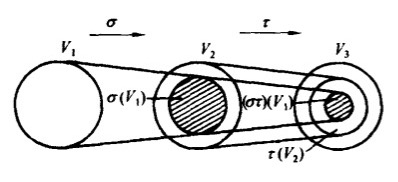
\includegraphics[scale=.5]{figs/5C.4.1.jpg}
          \end{figure}
          又因为 $ (\tau \sigma)(V_1) = \tau(\sigma(V_1)) $,所以又有
          \[ \dim(\tau \sigma)(V_1) \leqslant \dim \sigma(V_1) \]
          即 $ r(\tau \sigma) \leqslant r(\sigma) $.

          再证左边. 由线性映射维数公式,
          \begin{gather*}
              r(\tau) + \dim \ker \tau = n \\
              r(\tau \sigma) + \dim \ker(\tau \sigma) = m
          \end{gather*}
          又 $ \dim \ker(\tau \sigma) \leqslant \dim \ker \tau $,所以
          \[ m - r(\tau \sigma) = \dim \ker(\tau \sigma) \leqslant \dim \ker \tau \]
          代入线性映射维数公式,得 $ \dim \ker \tau = n - r(\tau) \geqslant m - r(\sigma) $,即
          \begin{align*}
              r(\tau \sigma) & \geqslant m + r(\tau) - n         \\
                             & \geqslant r(\sigma) + r(\tau) - n
          \end{align*}
        \end{answer}

        \item 设$V_1$是有限维线性空间,$\sigma,\tau\in \mathcal{L}(V_1,V_2)$,则
        \[r(\sigma+\tau) \leqslant r(\sigma)+r(\tau).\]

        事实上前两题的结论在后续章节矩阵的秩中都会涉及,此处有兴趣的同学可以尝试从线性映射的角度理解这两个秩不等式. 如果无法找到合适方式,可以考虑化为矩阵进行证明.
        \begin{answer}
            证明:由于 $ \forall \beta \in (\sigma + \tau)(V_1),\enspace \exists \alpha \in V_1 $ 使 $ \beta = (\sigma + \tau)(\alpha) = \sigma(\alpha) + \tau(\alpha) \in \sigma(V_1) + \tau(V_1) $,所以
          \[ (\sigma + \tau)(V_1) \subseteq \sigma(V_1) + \tau(V_1) \]
          因此
          \begin{align*}
              \dim(\sigma + \tau)(V_1) & \leqslant \dim(\sigma(V_1) + \tau(V_1))     \\
                                       & \leqslant \dim \sigma(V_1) + \dim \tau(V_1)
          \end{align*}
        \end{answer}
        \item 设$\sigma\in \mathcal{L}(V,V)$,$\dim V=n$,且$\sigma^2=\sigma$,$I$是$V$上的恒等变换. 证明:
        \begin{enumerate}
            \item $(I-\sigma)(V) \subseteq \ker\sigma$;

            \item $r(I-\sigma)+r(\sigma)=n$.
        \end{enumerate}

        \begin{answer}
            \begin{enumerate}
                \item \label{item:5:C:6:1}
                      $ \forall \sigma \in \mathcal{L}(V, V) $,则 $ I - \sigma \in \mathcal{L}(V, V) $. $ \forall \alpha \in (I - \sigma)(V),\enspace \exists \beta \in V $,有
                      \begin{gather*}
                          \alpha = (I - \sigma)(\beta) = \beta - \sigma(\beta) \\
                          \sigma(\alpha) = \sigma(\beta - \sigma(\beta)) = \sigma(\beta) - \sigma^2(\beta)
                      \end{gather*}
                      而由于 $ \sigma^2 = \sigma $,所以 $ \sigma(\alpha) = \vec{0} $,于是 $ \alpha \in \ker \sigma $,因此 $ (I - \sigma)(V) \subseteq \ker \sigma $.

                \item 利用 $ r(\sigma + \tau) \leqslant r(\sigma) + r(\tau) $ 和 $ r(\sigma) + \dim \ker \sigma = n $,由 \ref*{item:5:C:6:1} 可得
                      \begin{equation} \label{eq:5:C:6:2:1}
                          r(I - \sigma) + r(\sigma) \leqslant n
                      \end{equation}
                      又因为
                      \begin{equation} \label{eq:5:C:6:2:2}
                          r(I - \sigma) + r(\sigma) \geqslant r(I - \sigma + \sigma) = r(I) = n
                      \end{equation}
                      于是由\autoref{eq:5:C:6:2:1} 和\autoref{eq:5:C:6:2:2} 即可得到 $ r(I - \sigma) + r(\sigma) = n $.
            \end{enumerate}
        \end{answer}


        \item 设$V$是一个$n$维线性空间,$\sigma\in \mathcal{L}(V,V)$,且$\sigma^2=\theta$(零映射). 证明:
        \begin{enumerate}
            \item $ \dim \im \sigma \leqslant \dfrac{n}{2} $;

            \item 设$A$是$\sigma$在某组基下的矩阵,则方程组$AX=0$的基础解系至少有$\dfrac{n}{2}$个解.
        \end{enumerate}
        \begin{answer}
            证明:\begin{enumerate}
                \item \label{item:5:C:7:1}
                      $ \forall \alpha \in \im \sigma,\enspace \exists \beta \in V $ 使得 $ \sigma(\beta) = \alpha $. 由 $ \sigma^2 = \theta $ 可得 $ \sigma(\alpha) = \sigma^2(\beta) = \vec{0} $,因此 $ \alpha \in \ker \sigma $,从而 $ \im \sigma \subseteq \ker \sigma $. 于是我们得到
                      \[ n = \dim \im \sigma + \dim \ker \sigma \geqslant 2 \dim \im \sigma \]
                      即 $ \dim \im \sigma \leqslant \dfrac{n}{2} $.

                \item 由 \ref*{item:5:C:7:1} 可知,方程组 $ AX = \vec{0} $ 的基础解系含有 $ n - r(A) = \dim \ker \sigma \geqslant \dfrac{n}{2} $ 个解向量,所以结论成立.
            \end{enumerate}

        \end{answer}
    \end{exgroup}
\end{exercise}
